% !TeX program = xelatex
% 中文期刊论文：按照南方电网技术投稿要求改写
% 编译建议：XeLaTeX。中文字体优先使用系统字体，缺失时回退到 TeX Live/CTeX 常见的 Fandol 字体。
\documentclass[UTF8,zihao=5,twoside]{ctexart}

\usepackage[a4paper,top=22mm,bottom=20mm,left=18mm,right=18mm,headheight=14pt,headsep=6mm,columnsep=7mm]{geometry}
\usepackage{fontspec}
\usepackage{xeCJK}
\usepackage{amsmath,amssymb,bm}
\usepackage{graphicx}
\usepackage{float}
\usepackage{booktabs,array,multirow,tabularx}
\usepackage{caption}
\usepackage{titlesec}
\usepackage{fancyhdr}
\usepackage{indentfirst}
\usepackage{enumitem}
\usepackage{multicol}
\usepackage{balance}
\usepackage{tikz}
\usetikzlibrary{arrows.meta,positioning,shapes.geometric}
\usepackage[hidelinks]{hyperref}

\graphicspath{{figures/}}

% -------------------- 字体 --------------------
\IfFontExistsTF{Songti SC}
  {\setCJKmainfont{Songti SC}}
  {\IfFontExistsTF{SimSun}
    {\setCJKmainfont{SimSun}}
    {\setCJKmainfont{FandolSong-Regular.otf}[BoldFont=FandolSong-Bold.otf,ItalicFont=FandolKai-Regular.otf]}}
\IfFontExistsTF{Heiti SC}
  {\setCJKsansfont{Heiti SC}}
  {\IfFontExistsTF{SimHei}
    {\setCJKsansfont{SimHei}}
    {\setCJKsansfont{FandolHei-Regular.otf}[BoldFont=FandolHei-Bold.otf]}}
\IfFontExistsTF{Kaiti SC}
  {\setCJKfamilyfont{kai}{Kaiti SC}}
  {\IfFontExistsTF{KaiTi}
    {\setCJKfamilyfont{kai}{KaiTi}}
    {\setCJKfamilyfont{kai}{FandolKai-Regular.otf}}}
\IfFontExistsTF{Times New Roman}{\setmainfont{Times New Roman}}{\IfFontExistsTF{TeX Gyre Termes}{\setmainfont{TeX Gyre Termes}}{\setmainfont{Latin Modern Roman}}}
\IfFontExistsTF{Arial}{\setsansfont{Arial}}{\IfFontExistsTF{TeX Gyre Heros}{\setsansfont{TeX Gyre Heros}}{\setsansfont{Latin Modern Sans}}}
\newcommand{\kaiti}{\CJKfamily{kai}}

\zihao{5}
\setlength{\parindent}{2em}
\linespread{1.08}
\setlist{nosep,leftmargin=2em}
\setlength{\textfloatsep}{0.7em plus 0.2em minus 0.2em}
\setlength{\floatsep}{0.6em plus 0.2em minus 0.2em}
\setlength{\intextsep}{0.6em plus 0.2em minus 0.2em}
\renewcommand{\topfraction}{0.95}
\renewcommand{\bottomfraction}{0.85}
\renewcommand{\textfraction}{0.05}
\renewcommand{\floatpagefraction}{0.85}
\setcounter{topnumber}{4}
\setcounter{bottomnumber}{2}
\setcounter{totalnumber}{6}

% -------------------- 页眉页脚 --------------------
\pagestyle{fancy}
\fancyhf{}
\fancyhead[LE]{\zihao{-5}第~\thepage~页}
\fancyhead[CE]{\zihao{-5}南方电网技术}
\fancyhead[RE]{\zihao{-5}第~XX~卷}
\fancyhead[LO]{\zihao{-5}\thepage}
\fancyhead[CO]{\zihao{-5}南方电网技术}
\fancyhead[RO]{\zihao{-5}第~XX~卷}
\renewcommand{\headrulewidth}{0.4pt}
\renewcommand{\footrulewidth}{0pt}

% -------------------- 标题层级 --------------------
\titleformat{\section}{\sffamily\zihao{4}\bfseries}{\thesection}{0.6em}{}
\titleformat{\subsection}{\sffamily\zihao{5}\bfseries}{\thesubsection}{0.6em}{}
\titleformat{\subsubsection}{\sffamily\zihao{5}\bfseries}{\thesubsubsection}{0.6em}{}
\titlespacing*{\section}{0pt}{0.8em}{0.4em}
\titlespacing*{\subsection}{0pt}{0.6em}{0.3em}
\titlespacing*{\subsubsection}{0pt}{0.4em}{0.2em}

% -------------------- 图表与公式 --------------------
\captionsetup{font={small},labelfont=bf,labelsep=quad,justification=centering}
\renewcommand{\figurename}{图}
\renewcommand{\tablename}{表}
\numberwithin{equation}{section}
\renewcommand{\theequation}{\arabic{equation}}

\newcommand{\figbicaption}[2]{%
  \caption{#1\\[-0.2em]\small Fig.\,\thefigure\ #2}
}
\newcommand{\tabbicaption}[2]{%
  \caption{#1\\[-0.2em]\small Tab.\,\thetable\ #2}
}
\newcommand{\metric}[1]{\mathrm{#1}}
\newcommand{\code}[1]{\texttt{#1}}

% -------------------- 参考文献格式 --------------------
\renewcommand{\refname}{参考文献}
\makeatletter
\renewenvironment{thebibliography}[1]{%
  \section*{\refname}%
  \small
  \list{[\arabic{enumi}]}{%
    \settowidth\labelwidth{[#1]}%
    \leftmargin\labelwidth
    \advance\leftmargin\labelsep
    \usecounter{enumi}}
  \sloppy\clubpenalty4000\widowpenalty4000\sfcode`\.\ \@m
}{\def\@noitemerr{\@latex@warning{Empty `thebibliography' environment}}\endlist}
\makeatother

\newcommand{\articleinfo}{文章编号：1674-0629(20XX)XX-XXXX-XX\quad 中图分类号：TM73\quad 文献标志码：A\\
DOI：10.13648/j.cnki.issn1674-0629.20XX.XX.XXX}

\newcommand{\fundcn}{基金项目：无。}
\newcommand{\funden}{Foundation item: None.}

\begin{document}
\twocolumn[

% ==================== 首页题名与摘要：单栏 ====================
\begin{center}
{\zihao{-5}\articleinfo}\par\vspace{1.0em}
{\sffamily\zihao{2}\bfseries 基于多相关性筛选与 L1 门控深度神经网络的电力数据隐性推断源定位}\par\vspace{0.8em}
{\zihao{4}杜浩存}\par\vspace{0.4em}
{\zihao{5}（西安交通大学 网络空间安全学院，陕西 西安 710049）}\par\vspace{0.8em}
\end{center}

\noindent\textbf{摘要：}电力系统运行与市场数据由物理约束、调度策略和市场出清机制共同生成，字段之间存在复杂且稳定的统计关联。为从高维字段中识别对目标变量具有主要推断贡献的紧凑字段集合，提出一种融合多相关性筛选与 L1 门控深度神经网络的隐性推断源定位方法。首先，利用 Pearson、Spearman、Kendall 相关系数以及归一化互信息、距离相关系数和 HSIC 六类指标进行多维度初筛；然后，在深度神经网络输入端引入可学习门控向量，并施加 L1 正则化约束压缩冗余字段；进一步构建相关性驱动的改进门控模型，将六类指标映射为统一门控判定边界。基于美国 PJM 电力市场 2025 年小时级公开数据开展实验，结果表明：以净实际交换功率为目标，L1 门控从 55 个候选字段中筛选出 18 个活跃字段，以此训练的普通深度神经网络验证 $R^2$ 达到 0.9681，高于全量字段的 0.9661；在 12 个目标变量上，L1 门控模型平均使用 15.5 个字段，字段利用率约为 22.46\%，平均测试 $R^2$ 为 0.9111，高于全量模型的 0.9031。同预算对比和冗余输入分析验证了所提方法在字段压缩、推断能力保持与关联解释方面的有效性。\par
\noindent\textbf{关键词：}电力数据分析；隐性推断源；相关性分析；L1 门控神经网络；特征选择；数据共享\par\vspace{0.8em}

\begin{center}
{\bfseries\large Implicit Inference-Source Localization for Power Data Based on Multi-Correlation Screening and L1-Gated Deep Neural Network}\par\vspace{0.5em}
{DU Haocun}\par\vspace{0.3em}
{\small (School of Cyber Science and Engineering, Xi'an Jiaotong University, Xi'an 710049, China)}\par\vspace{0.5em}
\end{center}

\noindent\textbf{Abstract:} Power system operation and market data are jointly shaped by physical constraints, dispatching strategies and market clearing mechanisms, giving rise to complex statistical dependencies among data fields. To identify a compact set of fields that makes major inference contributions to a target variable, this paper proposes an implicit inference-source localization method integrating multi-correlation screening with an L1-gated deep neural network. Six dependency measures, including Pearson, Spearman and Kendall correlation coefficients, normalized mutual information, distance correlation and HSIC, are employed for preliminary screening. A learnable gate vector with L1 regularization is then inserted at the DNN input layer to compress redundant fields. A correlation-driven improved gate further maps the six measures into a unified gate-decision boundary. Experiments on public 2025 PJM hourly market data show that, for net actual interchange, the L1 gate selects 18 active features from 55 candidates, and a standard DNN retrained on them achieves a test $R^2$ of 0.9681, higher than 0.9661 using all features. Across 12 target variables, the L1-gated model uses 15.5 features on average with a usage ratio of 22.46\% and an average test $R^2$ of 0.9111, exceeding 0.9031 for the full-feature model. Same-budget baseline comparisons and redundant-input analysis validate the effectiveness of the proposed method.\par
\noindent\textbf{Key words:} power data analysis; implicit inference source; correlation analysis; L1-gated neural network; feature selection; data sharing\par\vspace{0.8em}

\noindent{\small\fundcn\\\funden}
\vspace{0.8em}
]

\section{引言}
随着智能电网、广域测量和电力市场信息化建设的持续推进，电网运行过程中不断产生海量结构化数据。有效利用这些数据对运行评估、市场分析、调度决策和科研验证具有重要意义\cite{ref-liu-cps,ref-ma-pjm,ref-fan-pjm}。然而，电力系统数据的分析利用仍面临不同于一般工业数据的复杂性：其一，电网由大量互联节点、线路和设备构成，数据生成过程受到物理模型、运行约束和调度规则的共同影响；其二，运行、市场、负荷、发电和交换功率等数据与业务过程高度交织，不同数据类型之间的边界并不总是清晰；其三，电力数据体量大、字段多，而真正支撑目标变量分析的关键信息往往只分布在少量字段及其组合关系中。因此，如何在高维电力数据中识别具有主要推断贡献的字段集合，是数据价值挖掘、关联性分析和共享前评估中的基础问题。

从数据关联角度看，电力字段之间存在大量由物理规律和市场机制共同形成的显式或隐式联系。例如，负荷、发电结构、辅助服务容量、电价分量和区域交换功率等字段可能在不同时间尺度上表现出稳定的统计依赖。上述依赖一方面为运行状态理解和数据质量检查提供了依据，另一方面也意味着某些目标变量即使不直接作为模型输入，也可能被其他字段组合较好地恢复。对这类隐性关联进行分析，并不是简单追求预测精度，而是希望回答两个更具体的问题：哪些字段真正构成目标变量的主要推断源；在存在大量冗余字段的情况下，如何获得紧凑、可解释且具有稳定推断能力的字段集合。

现有相关性分析方法为字段关联发现提供了直接工具。Pearson 相关系数、Spearman 和 Kendall 秩相关系数已广泛应用于负荷预测、异常数据清洗和特征筛选等任务\cite{ref-lan-load,ref-jiao-pv,ref-deng-load}。为刻画非线性依赖关系，归一化互信息、距离相关系数\cite{ref-szekely-dcorr}和 HSIC\cite{ref-gretton-hsic}等指标也常被用于复杂数据关系识别。相关性方法具有计算效率高和结果直观的优点，适合在大规模字段空间中进行初步分析。然而，单一相关性指标只能覆盖特定数学意义下的两两依赖关系，难以同时描述线性、单调、非单调和高阶非线性耦合；同时，统计相关强弱并不等同于字段在联合推断模型中的实际贡献，若只依据相关性排序，容易忽略多个字段组合后的互补作用。

机器学习模型能够进一步检验字段集合对目标变量的联合推断能力。深度神经网络、随机森林\cite{ref-breiman-rf}和 XGBoost\cite{ref-chen-xgboost}等模型已在电力数据分析中得到广泛应用\cite{ref-wang-meter}。这类模型能够直接刻画复杂非线性映射，但全量输入模型通常只能说明目标变量整体可被预测，难以定位主要推断源字段。Lasso\cite{ref-tibshirani-lasso}和 ElasticNet\cite{ref-zou-enet}等稀疏线性模型具有变量选择能力，但表达能力受限于线性假设；树模型重要性排序则易受冗余字段和训练随机性的影响。文献\cite{ref-xing-micdnn}提出的 MIC-DNN 思路将信息系数与深度模型结合用于电力数据相关性验证，说明统计依赖与深度推断结合具有可行性，但在多字段联合场景下，仍需进一步解决推断源定位和冗余字段压缩问题。

综上，电力数据隐性推断源定位需要同时兼顾候选覆盖和冗余压缩。若初筛过窄，可能遗漏非线性或互补型关联字段；若直接使用全量字段训练深度模型，又会引入大量冗余输入，使结果难以解释，并可能削弱模型泛化能力。基于此，本文提出融合多相关性筛选与 L1 门控深度神经网络的电力数据隐性推断源定位方法。主要贡献如下：

1）构建了面向电力运行与市场数据的隐性推断源定位框架，将多相关性初筛、非线性推断建模、稀疏字段选择和再训练验证组织为统一流程，用于从高维候选字段中定位紧凑的推断源集合。

2）设计了基于六类相关性指标的保守初筛机制，并在深度神经网络输入端引入 L1 门控层，使字段选择由统计依赖证据和推断误差共同驱动，从而在保留主要推断路径的同时压缩冗余字段。

3）提出相关性驱动的改进门控模型，将六维相关性向量映射为门控值，并通过 Sigmoid 函数形成统一判定边界；基于 PJM 2025 年小时级公开数据开展单目标、多目标、同预算 baseline 及冗余输入实验，验证所提方法在字段压缩、推断能力保持和关联解释方面的有效性。

\section{隐性推断源定位方法}
\subsection{问题定义}
给定电力数据集
\begin{equation}
D=\{X_1,X_2,\ldots,X_w,Y\},
\end{equation}
其中 $Y\in\mathbb{R}^{n}$ 为待分析目标字段，$X_i\in\mathbb{R}^{n}$ 为候选字段，$w$ 为候选字段总数，$n$ 为样本数。在电力数据分析场景中，$Y$ 可以表示交换功率、电价、备用容量、负荷或其他具有业务分析价值的目标变量，$X_i$ 则表示与其处于同一运行或市场过程中的相关字段。若部分 $X_i$ 能够对 $Y$ 建立有效推断模型，说明这些字段共同包含了支撑目标变量恢复的主要关联信息。

本文关注的不是一般意义上的预测精度提升，而是字段级推断源定位问题。其目标是在候选字段中识别一个规模尽可能小的集合 $\mathcal{S}$，使其对目标字段 $Y$ 仍能维持较高推断精度：
\begin{equation}
\mathcal{S}^{*}=\arg\min_{\mathcal{S}\subseteq \{X_i\}}\left|\mathcal{S}\right|,
\quad
R^2(f_{\theta}(\mathcal{S}),Y)\geq \eta .
\end{equation}
式中：$f_{\theta}$ 为推断模型；$\eta$ 为可接受的推断能力阈值。$\mathcal{S}^{*}$ 的规模越小，说明目标字段越可能由少量字段组合恢复；若 $\mathcal{S}^{*}$ 中的字段具有明确业务含义，则可进一步用于解释变量关联、辅助字段分级和指导数据共享策略。模型推断性能采用决定系数 $R^2$ 衡量：
\begin{equation}
R^2=1-\frac{\sum_{k=1}^{n}(y_k-\hat{y}_k)^2}{\sum_{k=1}^{n}(y_k-\bar{y})^2}.
\end{equation}
式中：$y_k$ 为真实值；$\hat{y}_k$ 为模型预测值；$\bar{y}$ 为真实值的均值。当一个规模较小的字段集合所取得的 $R^2$ 接近或超过全量字段的结果时，表明该集合保留了主要推断路径；反之，当被剔除字段单独推断能力显著下降时，则表明这些字段主要贡献冗余信息或噪声。为避免把由显式公式或直接业务定义导致的关系误判为隐性关联，实验中对目标字段存在直接因果或构造关系的字段进行预先排除，随后再对剩余候选字段开展统计依赖和推断能力分析。

本文方法的总体流程如图~\ref{fig:method_flow} 所示。首先，对原始电力数据进行目标字段设定、候选字段整理和直接关系排除；其次，计算候选字段与目标字段之间的六类相关性指标，并采用宽松规则完成初筛；再次，将初筛后的字段送入 L1 门控深度推断模型，通过预测损失和稀疏惩罚共同学习活跃推断源；最后，使用普通 DNN 对选中字段进行再训练验证，并结合门控值、相关性权重和 baseline 对比结果解释字段贡献。该流程将统计分析与推断建模分工处理：相关性初筛负责提高候选覆盖率，门控模型负责压缩冗余并定位推断路径，再训练验证负责避免把门控层自身的训练偏差误认为字段贡献。

\begin{figure}[!tbp]
\centering
\includegraphics[width=\columnwidth]{总流程.png}
\figbicaption{隐性推断源定位总体流程}{Overall workflow of implicit inference-source localization}
\label{fig:method_flow}
\end{figure}

\subsection{多相关性初筛}
相关系数是刻画变量间关联关系的常用统计工具，其基本思想是将两个变量之间的同步变化程度、排序一致性、分布依赖或核空间依赖压缩为一个可比较的数值。对于高维电力数据分析而言，相关系数具有两个优点：一是计算效率高，可在大量字段上快速执行；二是结果具有较好的可解释性，便于对候选字段进行初步排序和筛查。但是，相关系数本质上属于描述性统计量，只能说明变量之间存在某种关联，不能直接证明某个字段在联合推断模型中不可替代。因此，本文将相关性分析定位为候选空间压缩和关联线索发现，而不是最终字段判定。

电力数据字段之间的依赖关系具有多样性：既可能因潮流方程、功率平衡或数据聚合形成近似线性关系，也可能因市场出清机制、辅助服务约束和分段调度规则产生复杂的非线性耦合。为降低单一统计指标造成的漏筛可能性，本文构建六维相关性向量对每个候选字段 $X_i$ 进行综合评估：
\begin{equation}
R_i=[r_i^{(\metric{NMI})},r_i^{(\metric{Spear})},r_i^{(\metric{Pear})},
r_i^{(\metric{Ken})},r_i^{(\metric{DC})},r_i^{(\metric{HSIC})}].
\end{equation}
式中：六个分量分别对应归一化互信息（NMI）、Spearman 秩相关系数、Pearson 相关系数、Kendall 秩相关系数、距离相关系数（DC）和 Hilbert-Schmidt 独立性准则（HSIC）。六类指标的作用侧重点不同。

Pearson 相关系数度量两个变量之间的线性相关程度，其定义为
\begin{equation}
\rho_{p}(X_i,Y)=
\frac{\mathrm{cov}(X_i,Y)}{\sigma_{X_i}\sigma_Y}.
\end{equation}
当字段之间存在近似线性派生关系或同步波动时，Pearson 系数能够给出直接反映。Spearman 相关系数先将变量转换为秩序列，再计算秩序列的 Pearson 相关，适合刻画单调但非严格线性的关系。Kendall 秩相关系数基于样本对的一致序和逆序关系定义，能够从排序一致性的角度反映变量间关联，对异常值和局部非线性变化相对稳健。

归一化互信息从信息论角度度量变量之间共享信息量，能够发现非单调和非线性依赖。本文将互信息按变量熵进行归一化，使其落入可比较范围。距离相关系数基于样本间距离矩阵度量变量依赖，当且仅当变量独立时其理论值为 0，因而能够捕捉一般形式的非线性关系。HSIC 则将变量映射到再生核 Hilbert 空间中，通过核矩阵的相关性度量统计依赖，适合刻画复杂非线性耦合。本文同时采用上述六类指标，是因为电力数据中线性、单调、非单调和高阶非线性依赖往往并存，任何单一指标都难以覆盖全部潜在推断路径。

初筛流程如图~\ref{fig:screening_flow} 所示。对每个候选字段，先分别计算六类相关性得分，并将不同指标的得分与对应阈值比较；随后采用“任一指标通过即保留”的宽松策略，即当任意一个指标达到预设阈值时，该字段即被保留进入后续门控建模：
\begin{equation}
\max_j I\left(r_i^{(j)}\geq \mu_1^{(j)}\right)>0.
\end{equation}
式中：$I(\cdot)$ 为示性函数；$\mu_1^{(j)}$ 为第 $j$ 类指标的初筛阈值。该策略的设计原则是宁可保留部分弱冗余字段，也不在早期排除可能具有互补推断作用的字段。换言之，初筛阶段强调召回率和候选覆盖，而不追求最终字段集合的最小化。字段是否真正构成隐性推断源，需要在后续 L1 门控模型中由推断误差和稀疏约束共同决定。

\begin{figure}[!tbp]
\centering
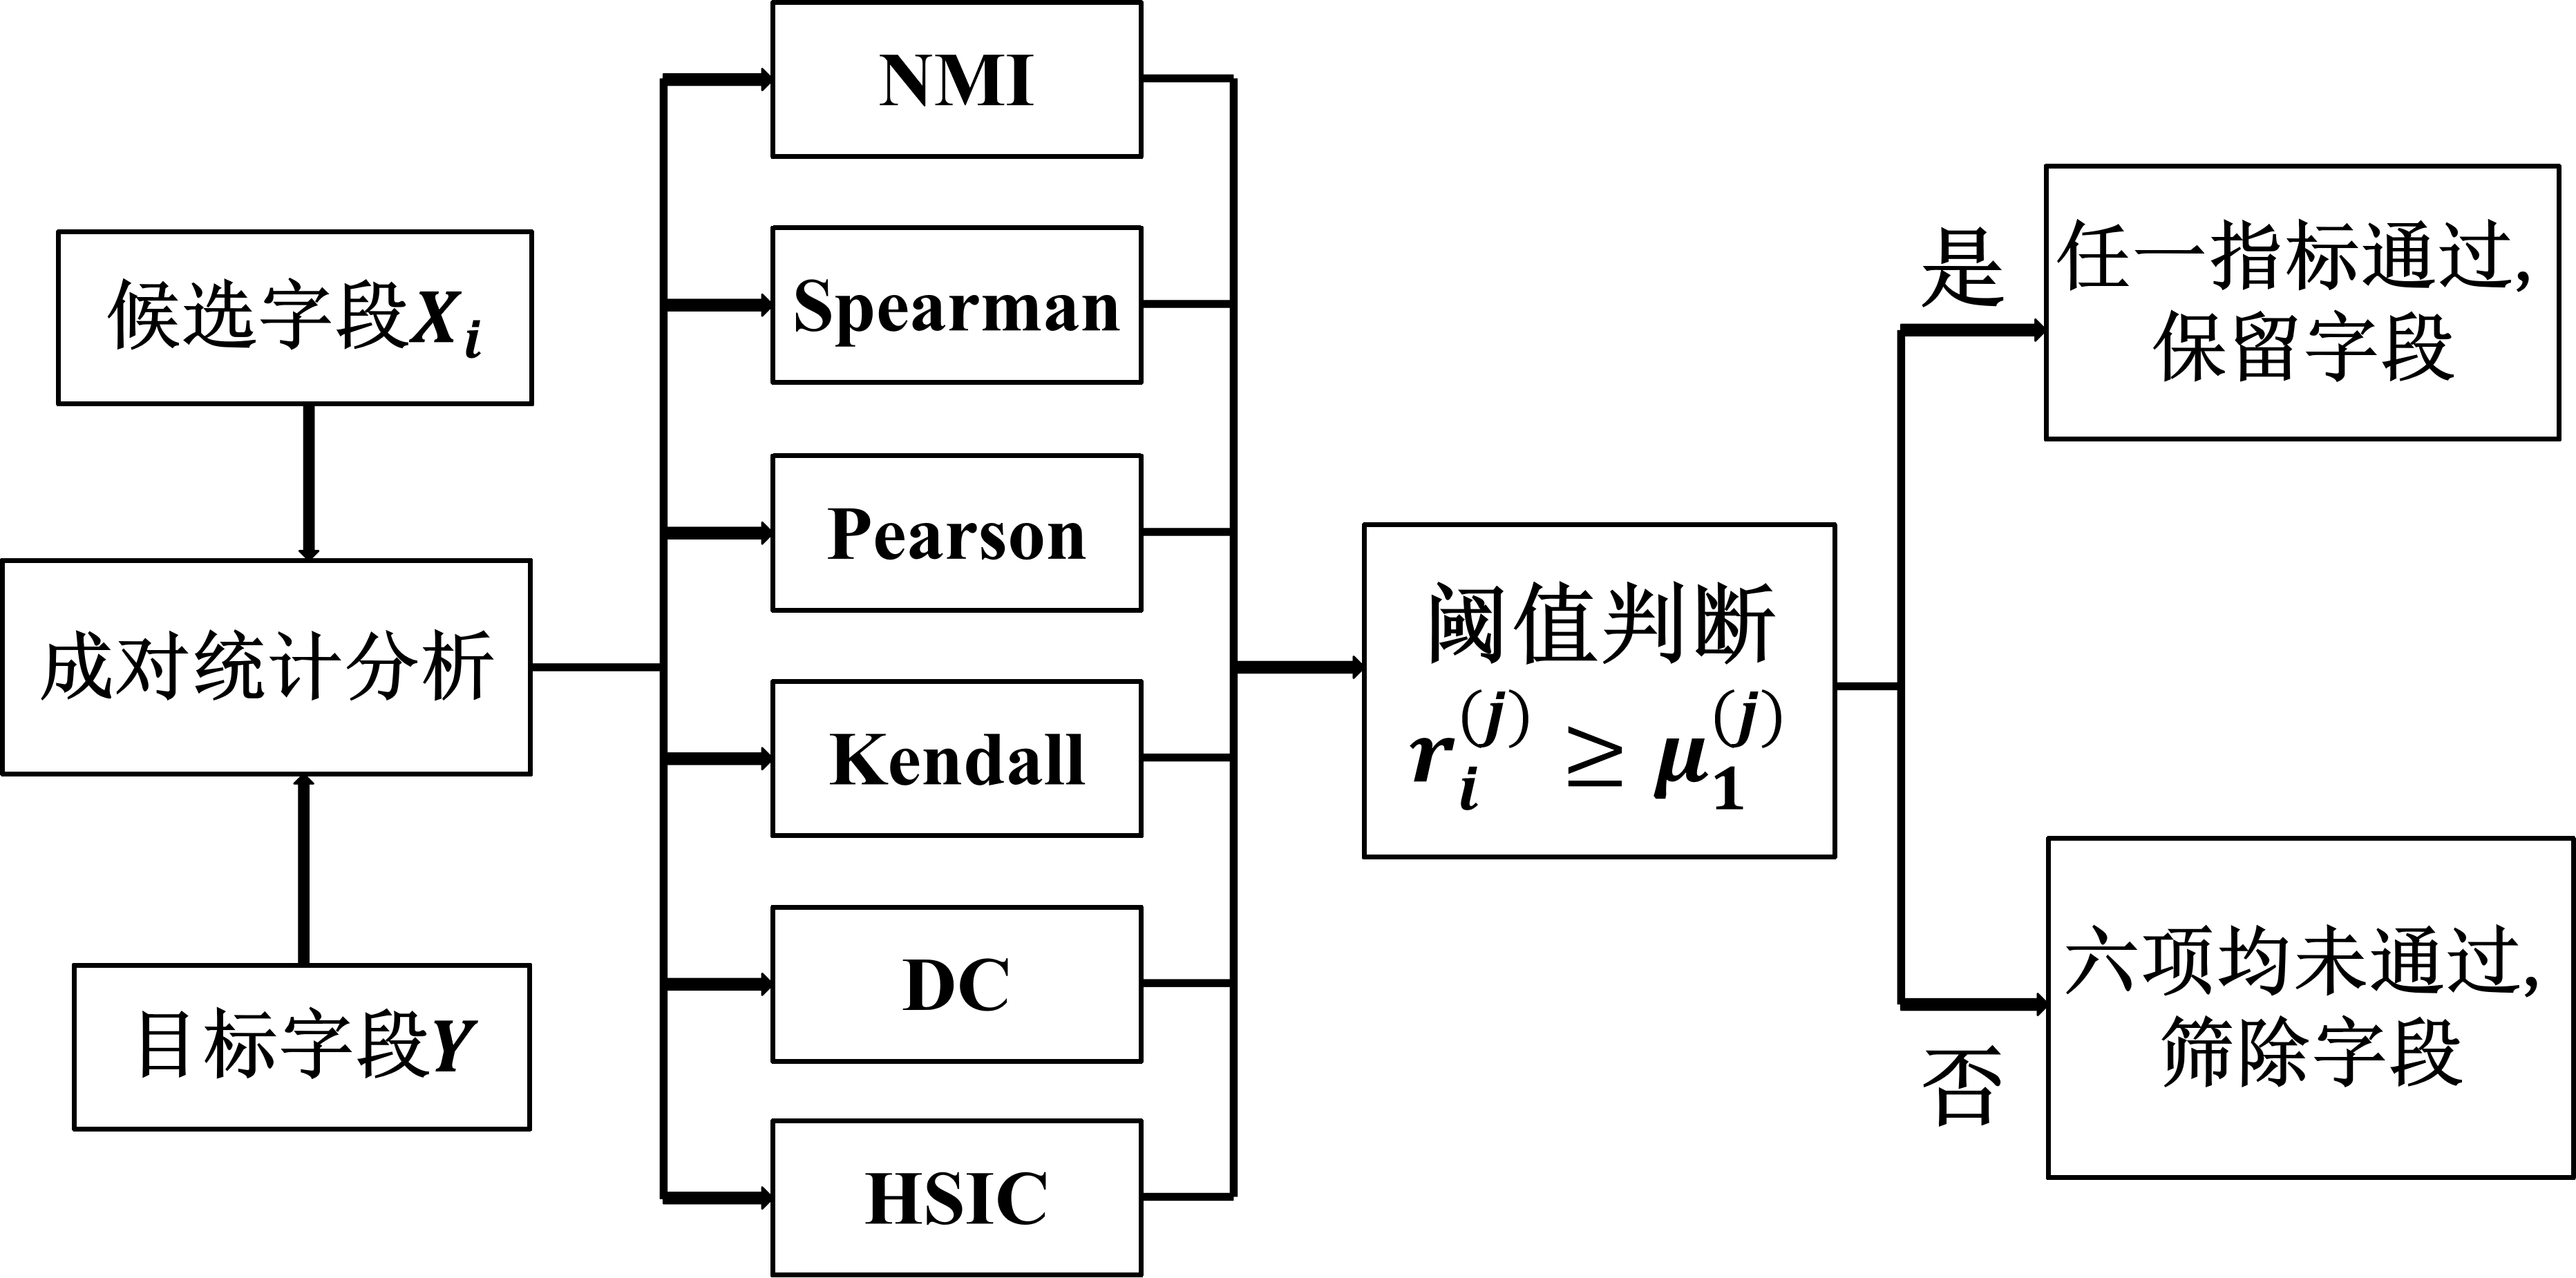
\includegraphics[width=\columnwidth]{初筛流程.png}
\figbicaption{多相关性初筛流程}{Multi-correlation preliminary screening workflow}
\label{fig:screening_flow}
\end{figure}

\subsection{L1 门控深度推断模型}
经过多相关性初筛后，得到候选字段集合 $X=\{X_1,\ldots,X_m\}$，其中 $m$ 为通过初筛的字段数。相关性初筛能够删除明显弱相关字段，但仍会保留大量在统计上有关联、在推断模型中却可能相互替代的字段。若直接使用全部初筛字段训练普通 DNN，模型虽然可能取得较高 $R^2$，但无法说明哪些输入字段承担主要推断作用。为此，本文在深度神经网络的输入端引入可学习门控层，其结构如图~\ref{fig:l1_structure} 所示。

\begin{figure}[!tbp]
\centering

\includegraphics[width=\columnwidth]{L1.png}
\figbicaption{L1 门控深度推断模型结构}{Structure of the L1-gated deep inference model}
\label{fig:l1_structure}
\end{figure}

设门控向量为 $g=[g_1,\ldots,g_m]$，其中 $g_i$ 与候选字段 $X_i$ 一一对应。门控层对输入字段进行逐元素加权，模型输出为
\begin{equation}
\hat{Y}=f_{\theta}(g\odot X),
\end{equation}
式中：$\odot$ 为逐元素相乘运算；$f_{\theta}$ 为由多层全连接网络构成的非线性推断模型。当 $g_i$ 较大时，字段 $X_i$ 的信息能够较充分地进入后续网络；当 $g_i$ 接近 0 时，该字段在前向传播中被显著抑制。为了使门控值既服务于推断精度，又能够产生稀疏选择结果，训练目标函数定义为
\begin{equation}
\mathcal{L}=\frac{1}{n}\sum_{k=1}^{n}(y_k-\hat{y}_k)^2+\lambda\sum_{i=1}^{m}|g_i|.
\end{equation}
式中：第一项为均方误差损失，用于保证模型对目标字段的推断能力；第二项为 L1 正则化惩罚，$\lambda$ 为正则化系数，用于推动门控参数趋向稀疏。该目标函数体现了字段选择中的竞争机制：若某字段能够稳定降低预测误差，反向传播会保留或增大其门控值；若某字段主要提供重复信息、弱相关扰动或噪声，L1 惩罚会持续压低其门控值。与先训练模型再事后解释特征重要性不同，L1 门控将字段筛选嵌入推断模型训练过程，使字段取舍直接受到目标推断误差约束。

训练结束后，满足
\begin{equation}
|g_i|\geq \mu_2
\end{equation}
的字段被判定为活跃推断源。式中 $\mu_2$ 为活跃阈值。本文将活跃字段数量记为 $n_s$，并在后续 baseline 对比实验中作为统一字段预算，使不同方法在相同字段数量约束下进行公平比较。为检验门控筛选结果是否独立有效，本文不直接把门控模型的训练结果作为最终结论，而是将选中字段重新输入普通 DNN 进行训练和测试。若再训练模型仍能保持较高 $R^2$，则说明该字段集合确实包含支撑目标字段推断的主要信息。

\subsection{相关性驱动的改进门控}
普通 L1 门控模型能够在推断训练过程中识别活跃字段，但每个门控参数都是独立学习的变量，尚不能直接回答“六种相关性指标分别对最终字段判定贡献多少”这一问题。前述六类相关性指标虽然提供了统计依赖证据，但在普通流程中主要用于初筛，其作用仍停留在描述性分析层面，没有与最终推断导向的门控判定形成统一融合机制。换言之，初筛阈值能够决定某个字段是否进入候选空间，却不能解释不同相关性指标如何共同影响门控打开或关闭。

这一问题在增量数据分析中更为突出。假设新增一列候选字段，若仍采用普通 L1 门控方法，通常需要把新字段并入候选集合并重新训练推断模型，才能判断其是否构成推断源。若能够学习出不同相关性指标对推断贡献的权重，则可先计算新字段与目标字段之间的六维相关性向量，再通过统一映射快速得到门控评分，从而降低增量字段评估的计算成本。基于这一考虑，本文进一步提出相关性驱动的改进门控模型，其结构如图~\ref{fig:improved_gate_structure} 所示。

\begin{figure}[!tbp]
\centering
\includegraphics[width=\columnwidth]{改进L1.png}
\figbicaption{相关性驱动的改进门控层结构}{Structure of the correlation-driven improved gate layer}
\label{fig:improved_gate_structure}
\end{figure}

改进门控不再为每个字段直接设置相互独立的自由门控参数，而是将字段 $X_i$ 的六维相关性向量 $R_i$ 作为门控生成依据，通过线性映射和 Sigmoid 激活函数得到门控值：
\begin{equation}
g_i=\sigma(W^{\mathrm{T}}R_i+b),
\end{equation}
式中：$W\in\mathbb{R}^{6}$ 为六类相关性指标对应的可学习权重向量，反映各指标对推断源判定的相对贡献；$b$ 为全局偏置项，可理解为整体门控打开难度；$\sigma(\cdot)$ 为 Sigmoid 激活函数：
\begin{equation}
\sigma(z)=\frac{1}{1+\mathrm{e}^{-z}}.
\end{equation}
Sigmoid 函数将任意实数映射到 $(0,1)$ 区间，使门控值可以解释为字段被打开的连续强度。当 $z$ 较大时，$\sigma(z)$ 接近 1，字段信息被保留；当 $z$ 较小时，$\sigma(z)$ 接近 0，字段信息被抑制。更重要的是，Sigmoid 在 $z=0$ 处的输出恰好为 0.5，因此当 $W^{\mathrm{T}}R_i+b=0$ 时，$g_i=0.5$。这一性质使 0.5 不再是经验指定的阈值，而是由门控函数形式自然给出的开闭分界点，对应如下门控边界方程：
\begin{equation}
W^{\mathrm{T}}R_i+b=0.
\end{equation}
当 $g_i>0.5$ 时，说明字段 $X_i$ 的综合相关性证据位于门控打开侧，该字段更可能作为潜在推断源进入模型；当 $g_i<0.5$ 时，说明其综合证据不足以支持门控打开，该字段更可能为冗余或低贡献字段。训练过程中，$W$、$b$ 与 DNN 主干参数共同优化，并受到推断误差和门控稀疏约束的共同影响。因此，$W$ 的大小不仅反映某类相关性指标的统计强弱，还反映该指标在当前目标推断任务中的有效贡献。

与普通 L1 门控相比，改进门控的主要价值并不在于单纯追求更高的 $R^2$，而在于把“多种相关性证据如何共同形成字段判定”转化为可学习的统一边界。对于已有字段，模型能够解释不同相关性指标对门控开闭的贡献；对于新进入的数据字段，若其与目标字段之间的六维相关性已知，则可通过 $g_i=\sigma(W^{\mathrm{T}}R_i+b)$ 快速计算门控评分，在不立即重训完整推断模型的情况下获得初步判定。这种设计使相关性分析从独立初筛工具进一步转化为推断导向的统一边界表达。

\section{实验与结果分析}
\subsection{实验设置}
实验数据采用美国 PJM 互联电网 2025 年小时级公开市场与运行数据，数据路径为 \code{NEW\_PROJECT/data/processed/data2025\_Processed\_V2/}。PJM 数据虽然来源于公开市场平台，但其覆盖发电、负荷、电价、辅助服务和交换功率等典型电力业务环节，能够反映电力系统运行数据“字段多、机制耦合强、关联关系复杂”的共性特征。因此，本文将其作为公开可复现实验对象，用于验证所提方法对电力数据隐性关联和推断源字段的定位能力。

该数据集包含 8760 行（对应全年逐小时记录）和 72 列，其中前两列为 UTC 和东部时间的时间戳，仅用于时间对齐，不参与建模分析。去除时间字段后，剩余 70 个数据字段可按照 PJM Data Miner 官方数据源定义划分为如表~\ref{tab:data_overview} 所示的类别。数据涵盖发电与损耗、风电光伏出力、燃料类型发电、负荷预测与计量、调频市场、辅助服务市场、节点电价和交换功率等多个业务领域，字段间存在广泛的物理和市场机制关联。

\begin{table}[!tbp]
\centering
\scriptsize
\setlength{\tabcolsep}{2pt}
\tabbicaption{PJM 2025 数据字段分类概览}{Classification of PJM 2025 data fields}
\label{tab:data_overview}
\begin{tabularx}{\columnwidth}{c>{\raggedright\arraybackslash}p{0.40\columnwidth}X}
\toprule
编号 & Dataset & 中文说明 \\
\midrule
D1--D2 & Generation and EHV Losses & 小时级总发电量与超高压损耗数据。 \\
D3 & Wind Generation & PJM 区域小时级风电出力。 \\
D4 & Solar Generation & PJM 区域小时级光伏出力。 \\
D5--D24 & Generation by Fuel Type & 按燃料类型统计的发电出力与占比。 \\
D25--D26 & Historical Load Forecasts & 日前及最新可用负荷预测。 \\
D27 & Hourly Load: Preliminary & 由遥测数据计算的预估小时负荷。 \\
D28 & Hourly Load: Metered & PJM RTO 服务区域计量负荷。 \\
D29--D37 & Regulation Billing Data & 调频市场预结算相关价格、容量与信用数据。 \\
D38--D56 & Day-Ahead AS Market Results & 日前辅助服务市场的价格、需求与容量结果。 \\
D57--D60 & Day-Ahead Hourly LMPs & 日前能量市场 LMP、拥塞价与边际损耗价。 \\
D61--D64 & Real-Time Hourly LMPs & 实时能量市场 LMP、拥塞价与边际损耗价。 \\
D65--D70 & Actual/Schedule Summary & 净/总实际、计划和非计划交换功率。 \\
\bottomrule
\end{tabularx}
\end{table}

\subsubsection{参数设置}
多相关性初筛阶段的各项阈值设置如下：归一化互信息（NMI）为 0.06、Spearman 秩相关系数为 0.15、Pearson 相关系数为 0.15、Kendall 秩相关系数为 0.12、距离相关系数为 0.20、HSIC 为 0.25。上述阈值均用于"任一指标通过即保留"的宽松初筛规则。深度神经网络主干结构采用三层全连接隐藏层，各层神经元数量依次为 64、32 和 16；优化器采用 Adam；批次大小设为 50；训练轮数为 200；随机种子固定为 42 以保证实验可重复性。普通 L1 门控模型的 L1 正则化系数 $\lambda$ 设为 0.002，活跃阈值 $\mu_2$ 设为 0.10。改进 L1 门控模型的门控判定阈值为 0.50，L1 正则化系数设为 0.016，权重向量 $W$ 和偏置 $b$ 分别配置独立学习率，以确保相关性权重和门控偏置的稳定收敛。

\subsubsection{对比方法}
为全面评估所提方法的有效性，本文设计了三组对比实验。

第一组为全量模型与 L1 门控模型的直接对比。全量 DNN 使用当前目标允许的全部候选字段进行训练，L1DNN 则先由 L1 门控模型获取活跃字段集合，再以相同的 DNN 结构重新训练并评估推断性能。该组对比旨在验证 L1 门控在字段压缩后是否仍能保持甚至提升推断能力。

第二组为同预算 baseline 对比。具体而言，先利用 L1 门控模型在不同特征预算序列上搜索，确定使其 $R^2$ 达到全量 DNN 的 95\% 或 97\% 水平时所需的字段数 $n$；随后分别采用 NMI、Pearson、Spearman 排序选择、Lasso、ElasticNet、随机森林和 XGBoost 的特征重要性排序，在相同字段数 $n$ 下各自选取 Top-n 字段，并统一使用普通 DNN 训练和测试。该组对比消除了字段数量差异的影响，使比较聚焦于不同方法的字段选择质量。

第三组为冗余噪声影响分析实验。通过比较全量字段、L1 选中字段和不同 Top-n 字段的训练曲线与测试 $R^2$，分析少量字段推断精度优于全量字段的内在原因，揭示冗余噪声对模型泛化性能的影响机制。

\subsection{单目标关联推断源定位}
\subsubsection{多相关性初筛结果}
以净实际交换功率（\code{net\_actual\_interchange\_mw}）为中心目标，在剔除与之存在直接因果关系的净计划交换功率和总发电量后，共有 67 个候选关系参与初筛分析。经六类指标综合评估后，保留 55 个候选字段，筛除 12 个与目标明显弱相关的字段。各类指标的通过数量分别为：NMI 23 个、Spearman 33 个、Pearson 25 个、Kendall 29 个、距离相关系数 27 个、HSIC 31 个。各字段通过指标数的分布情况为：0 项（即被筛除）12 个、1 项 19 个、2 项 5 个、3 项 5 个、4 项 10 个、5 项 12 个、6 项（全部通过）4 个。

表~\ref{tab:screening_top} 按最大绝对相关得分从高到低给出初筛结果的节选。可以观察到，辅助服务市场字段、交换功率相关字段和燃料结构字段在多类指标下均表现出较强的统计依赖性，表明净实际交换功率的潜在推断路径涉及多个业务领域，并非由单一线性相关关系所决定。

\begin{table}[!tbp]
\centering
\scriptsize
\setlength{\tabcolsep}{1pt}
\tabbicaption{净实际交换功率目标的多相关性初筛结果节选}{Partial multi-correlation screening results for net actual interchange}
\label{tab:screening_top}
\begin{tabularx}{\columnwidth}{cXrrrrrrc}
\toprule
排名 & 字段 & NMI & Spear. & Pear. & Kend. & DC & HSIC & 通过数 \\
\midrule
1 & 30 min备用实际量 & 0.076 & -0.430 & -0.394 & -0.289 & 0.403 & 0.856 & 6 \\
2 & 30 min备用总量 & 0.067 & -0.428 & -0.397 & -0.252 & 0.374 & 0.845 & 6 \\
3 & 总计划交换功率 & 0.133 & -0.465 & -0.483 & -0.318 & 0.458 & 0.813 & 6 \\
4 & 核电出力 & 0.116 & -0.354 & -0.424 & -0.248 & 0.442 & 0.795 & 6 \\
\multicolumn{9}{c}{\(\cdots\)} \\
53 & 实时拥塞价 & 0.013 & 0.124 & 0.155 & 0.091 & 0.182 & 0.032 & 1 \\
54 & 同步备用MCP & 0.050 & 0.175 & 0.133 & 0.111 & 0.134 & 0.063 & 1 \\
55 & 日前拥塞价 & 0.073 & -0.039 & -0.066 & -0.048 & 0.171 & 0.070 & 1 \\
\bottomrule
\end{tabularx}
\end{table}

\subsubsection{推断精度与门控收缩过程}
图~\ref{fig:train_pair} 对比展示了净实际交换功率目标上全量 DNN 和 L1 门控模型的训练过程。全量 DNN 在 55 个候选字段上训练，最优测试 $R^2$ 为 0.9675；L1 门控模型在同一候选空间中训练，最优测试 $R^2$ 达到 0.9775。结果表明，稀疏门控约束不仅未削弱模型推断能力，反而在当前数据划分下提升了泛化性能。其原因在于，L1 门控在训练过程中持续压缩冗余字段的贡献，迫使模型更集中地利用稳定的推断路径，从而降低了过拟合倾向。

\begin{figure}[!tbp]
\centering
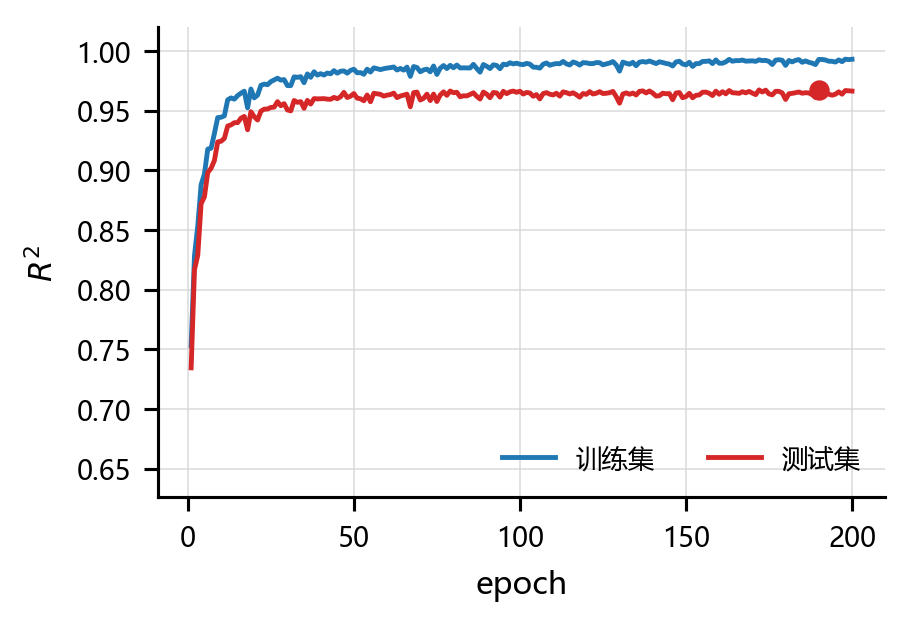
\includegraphics[width=\columnwidth]{net_train_dnn_r2_zh.png}\\[-0.2em]
{\scriptsize (a) 全量 DNN}\\[0.45em]
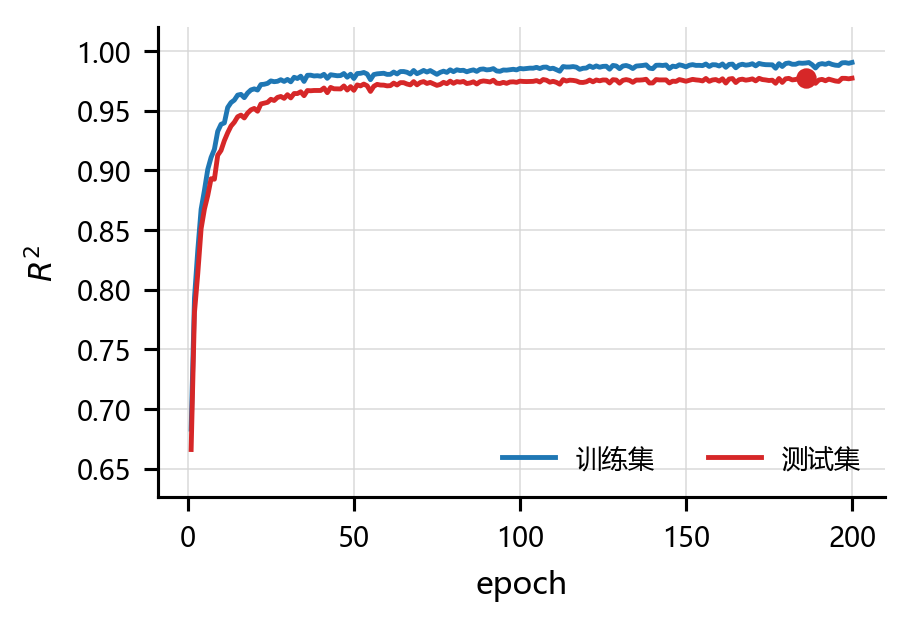
\includegraphics[width=\columnwidth]{net_train_l1_r2_zh.png}\\[-0.2em]
{\scriptsize (b) L1 门控模型}
\figbicaption{净实际交换功率目标上的 $R^2$ 训练过程对比}{Comparison of training $R^2$ processes for net actual interchange}
\label{fig:train_pair}
\end{figure}

图~\ref{fig:l1_gate} 展示了 L1 门控模型的门控参数演化过程，图中每条曲线对应一个候选字段的门控值随训练轮次的变化轨迹。在训练初期，各字段的门控值即出现明显分化；随着 L1 正则化惩罚的持续作用，大量弱贡献字段的门控值逐步衰减至阈值以下，仅有少数关键字段维持较高的门控值。在活跃阈值 $\mu_2=0.10$ 下，最终保留 18 个活跃字段，其中包含天然气发电出力、煤电出力、实时负荷、计量负荷、预估小时负荷和光伏发电出力等关键运行变量。图~\ref{fig:l1_active} 进一步展示了活跃字段数量随训练轮次的变化趋势，可以观察到活跃字段数量呈现逐步下降并趋于稳定的特征。这说明 L1 门控并非在训练结束时一次性截断弱字段，而是在优化过程中通过梯度信息逐步识别并剔除冗余字段，最终形成紧凑的推断源集合。

\begin{figure}[!tbp]
\centering

\includegraphics[width=\columnwidth]{net_l1_gate_params_zh.png}
\figbicaption{净实际交换功率目标上门控参数的演化过程}{Evolution of gate parameters for net actual interchange}
\label{fig:l1_gate}
\end{figure}

\begin{figure}[!tbp]
\centering

\includegraphics[width=\columnwidth]{net_l1_active_features_zh.png}
\figbicaption{净实际交换功率目标上活跃字段数量的变化}{Number of active features over training epochs}
\label{fig:l1_active}
\end{figure}

\subsubsection{Top-n 推断源验证}
为独立验证 L1 门控所选字段是否具备实际推断能力，本文按最终门控值从大到小排序，依次取 Top3、Top6、Top9、Top12、Top15、Top18 字段，分别训练普通 DNN 并评估其测试 $R^2$，同时与全量 55 字段和未选中 37 字段的结果进行比较。实验结果如图~\ref{fig:top_series} 所示。

当字段数较少时，推断能力受到明显限制：Top3 和 Top6 的测试 $R^2$ 分别仅为 0.4469 和 0.5778。随着字段数增加，推断能力显著提升：Top9 达到 0.9186，Top15 达到 0.9630，Top18 达到 0.9681，略高于全量 55 字段的 0.9661。与之形成对比的是，去除 Top18 后剩余的 37 个未选中字段单独训练仅取得 0.7820 的测试 $R^2$。上述结果表明，L1 门控识别出的字段集合具有两个重要特征：一是所选字段共同构成了支撑目标推断的核心路径，推断能力与甚至略优于全量字段；二是未选中字段尽管数量更多，但缺乏关键推断路径，单独推断能力显著下降。这进一步印证了 L1 门控不是简单挑选个别强相关字段，而是识别出能够联合支撑目标推断的非冗余字段组合。

\begin{figure}[!tbp]
\centering

\includegraphics[width=\columnwidth]{net_top_series_r2_zh.png}
\figbicaption{净实际交换功率目标上的 Top-n 推断源验证结果}{Top-n inference-source validation for net actual interchange}
\label{fig:top_series}
\end{figure}

\subsubsection{改进门控的门控边界学习}
图~\ref{fig:improved_gate} 至图~\ref{fig:improved_b} 展示了相关性驱动改进门控模型的训练结果。与普通 L1 门控模型不同，改进门控的门控值由六维相关性向量经 Sigmoid 映射生成，因此判定阈值设为 0.5，具有明确的数学含义：当 $W^{\mathrm{T}}R_i+b=0$ 时，Sigmoid 输出恰好为 0.5，对应门控边界；高于该边界表示相关性证据足以支持字段作为推断源，低于该边界则表示字段更可能为冗余或低贡献字段。

在本次实验中，改进 L1 门控最终保留 17 个活跃字段，最优测试 $R^2$ 为 0.9726。从权重向量 $W$ 的演化过程来看，HSIC 对应的权重在训练收敛后保持最高，表明非线性依赖证据对净实际交换功率目标的字段判定贡献最为显著；偏置 $b$ 从接近零的初始值逐步下降至约 $-0.70$，反映出模型在 L1 正则化压力下不断收紧门控打开条件。改进门控的核心意义在于：它将“各类统计指标如何共同影响字段判定”这一问题转化为可学习的统一边界，取代了传统方法中需要为每个指标独立设置阈值的方式。

\begin{figure}[!tbp]
\centering

\includegraphics[width=\columnwidth]{improved_l1_gate_params_zh.png}
\figbicaption{改进 L1 门控模型的门控值演化}{Gate value evolution of the improved L1-gated model}
\label{fig:improved_gate}
\end{figure}

\begin{figure}[!tbp]
\centering
\begin{minipage}{\columnwidth}
\centering
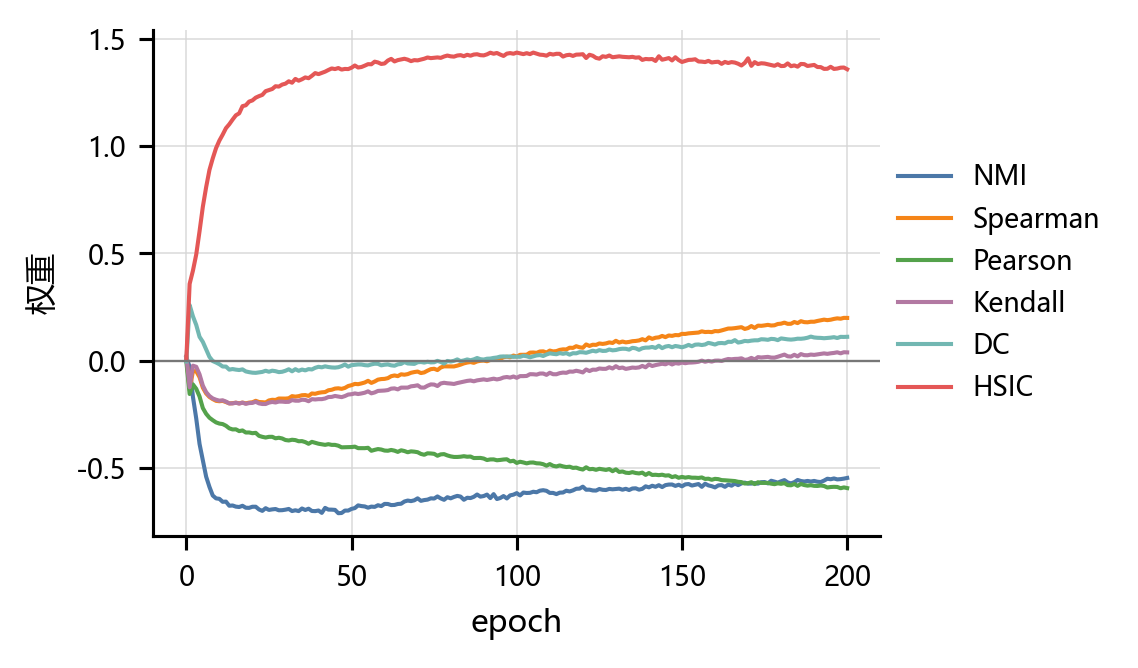
\includegraphics[width=0.92\linewidth]{improved_l1_w_meta_zh.png}\\[-0.4em]
{\scriptsize (a) 相关性指标权重 $W$ 的演化}
\end{minipage}\\[-0.2em]
\begin{minipage}{\columnwidth}
\centering

\includegraphics[width=0.86\linewidth]{improved_l1_b_meta_zh.png}\\[-0.4em]
{\scriptsize (b) 偏置 $b$ 的演化}
\end{minipage}
\figbicaption{改进门控中指标权重与偏置的训练演化}{Evolution of metric weights and bias in the improved gate}
\label{fig:improved_b}
\end{figure}

\subsection{多目标对比分析}
\subsubsection{全量模型与 L1 门控模型对比}
为系统评估所提方法的泛化性能，本文在 12 个目标变量上开展了全量 DNN 与 L1 门控选中特征 DNN 的直接对比实验。全量 DNN 使用当前目标允许的全部候选字段进行训练，L1DNN 则先由 L1 门控模型确定活跃字段集合，再使用相同网络结构重新训练并评估。实验结果如图~\ref{fig:dnn_l1_compare} 和表~\ref{tab:dnn_l1_compare} 所示。

以数据全集中 70 个数值字段扣除目标字段后的 69 个字段作为统一全量基准，全量 DNN 的字段利用率为 100\%，12 个目标的平均测试 $R^2$ 为 0.9031；L1 门控模型平均仅使用 15.50 个字段，字段利用率约为 22.46\%，平均测试 $R^2$ 为 0.9111，高于全量 DNN 的结果。从各目标的具体表现来看，在日前拥塞价、主备用容量、总实际交换功率和净实际交换功率等目标上，L1 门控模型显著或略微优于全量 DNN；在实时拥塞价和日前 LMP 上，L1 门控模型略低于全量 DNN。上述结果表明，所提方法并非对所有目标进行机械式的字段压缩，而是能够在大多数目标上以显著缩减的字段规模保持同等甚至更优的泛化能力。对于少数字段压缩后性能略有下降的目标，其下降幅度有限，仍处于可接受范围。

\begin{figure}[!tbp]
\centering

\includegraphics[width=\columnwidth]{dnn_vs_l1_method_compare_zh.png}
\figbicaption{12 个目标变量上全量 DNN 与 L1 门控模型的测试 $R^2$ 对比}{Comparison of test $R^2$ between all-feature DNN and L1-gated model across 12 targets}
\label{fig:dnn_l1_compare}
\end{figure}

\begin{table}[!tbp]
\centering
\scriptsize
\setlength{\tabcolsep}{2pt}
\tabbicaption{全量 DNN 与 L1 门控选中特征 DNN 的详细对比}{Detailed comparison between all-feature DNN and L1-gated selected-feature DNN}
\label{tab:dnn_l1_compare}
\begin{tabularx}{\columnwidth}{Xrrrr}
\toprule
中心目标 & 全量字段 & L1 字段 & 全量 DNN & L1DNN \\
\midrule
拥塞价 DA & 69 & 2 & 0.9408 & \textbf{0.9954} \\
主备用容量 & 67 & 14 & 0.8495 & \textbf{0.8826} \\
总实际交换 & 69 & 16 & 0.8499 & \textbf{0.8677} \\
30 min 备用容量 & 68 & 22 & 0.8967 & \textbf{0.9086} \\
边际损耗价 DA & 69 & 18 & 0.8936 & 0.8995 \\
净实际交换 & 67 & 18 & 0.9680 & 0.9728 \\
总发电量 & 42 & 16 & 0.9253 & 0.9271 \\
净计划交换 & 67 & 16 & 0.9691 & 0.9694 \\
总损耗 & 69 & 18 & 0.9413 & 0.9409 \\
计量负荷 & 42 & 15 & 0.9157 & 0.9139 \\
日前 LMP & 66 & 13 & \textbf{0.9622} & 0.9510 \\
拥塞价 RT & 69 & 18 & \textbf{0.7255} & 0.7040 \\
\midrule
平均 & -- & 15.5 & 0.9031 & 0.9111 \\
\bottomrule
\end{tabularx}
\end{table}

\subsubsection{同预算 baseline 对比}
为回应"baseline 的字段数 $n$ 是否由 L1 门控单方面决定"这一公平性问题，本文采用统一预算策略开展进一步对比。具体做法为：首先利用 L1 门控模型在特征预算序列上搜索，确定使其 $R^2$ 达到全量 DNN 的 95\% 或 97\% 水平时对应的字段数 $n$；若遍历候选预算后仍无法达到目标水平，则采用当前可获得的最优预算。随后，所有 baseline 方法在相同字段数 $n$ 下进行字段选择，并统一使用普通 DNN 训练和测试。在此设置下，不同方法的比较聚焦于"在相同字段预算下，谁选择的字段更具推断能力"，而非"谁使用了更多字段"。

图~\ref{fig:budget_lines} 给出了 95\% 和 97\% 统一预算下各目标的测试 $R^2$ 折线对比结果，图~\ref{fig:budget_avg} 进一步汇总了各方法在两种预算下的平均表现。在 95\% 预算水平下，平均字段数为 8.92，L1 门控模型的平均 $R^2$ 为 0.8875，高于随机森林的 0.8562、ElasticNet 的 0.8115、Lasso 的 0.7967 和 XGBoost 的 0.7798；在 97\% 预算水平下，平均字段数增加至 9.75，L1 门控模型的平均 $R^2$ 进一步提升至 0.8943，仍保持最优。在两种预算水平下，单相关性排序方法的整体表现偏低，表明仅依靠 NMI、Pearson 或 Spearman 等单一指标排序难以稳定保留联合推断所需的关键字段；树模型和线性稀疏模型虽在个别目标上具有竞争力，但在平均性能上仍不及 L1 门控模型。上述结果验证了所提方法在统一字段预算约束下的特征选择优势。

\begin{figure}[!tbp]
\centering
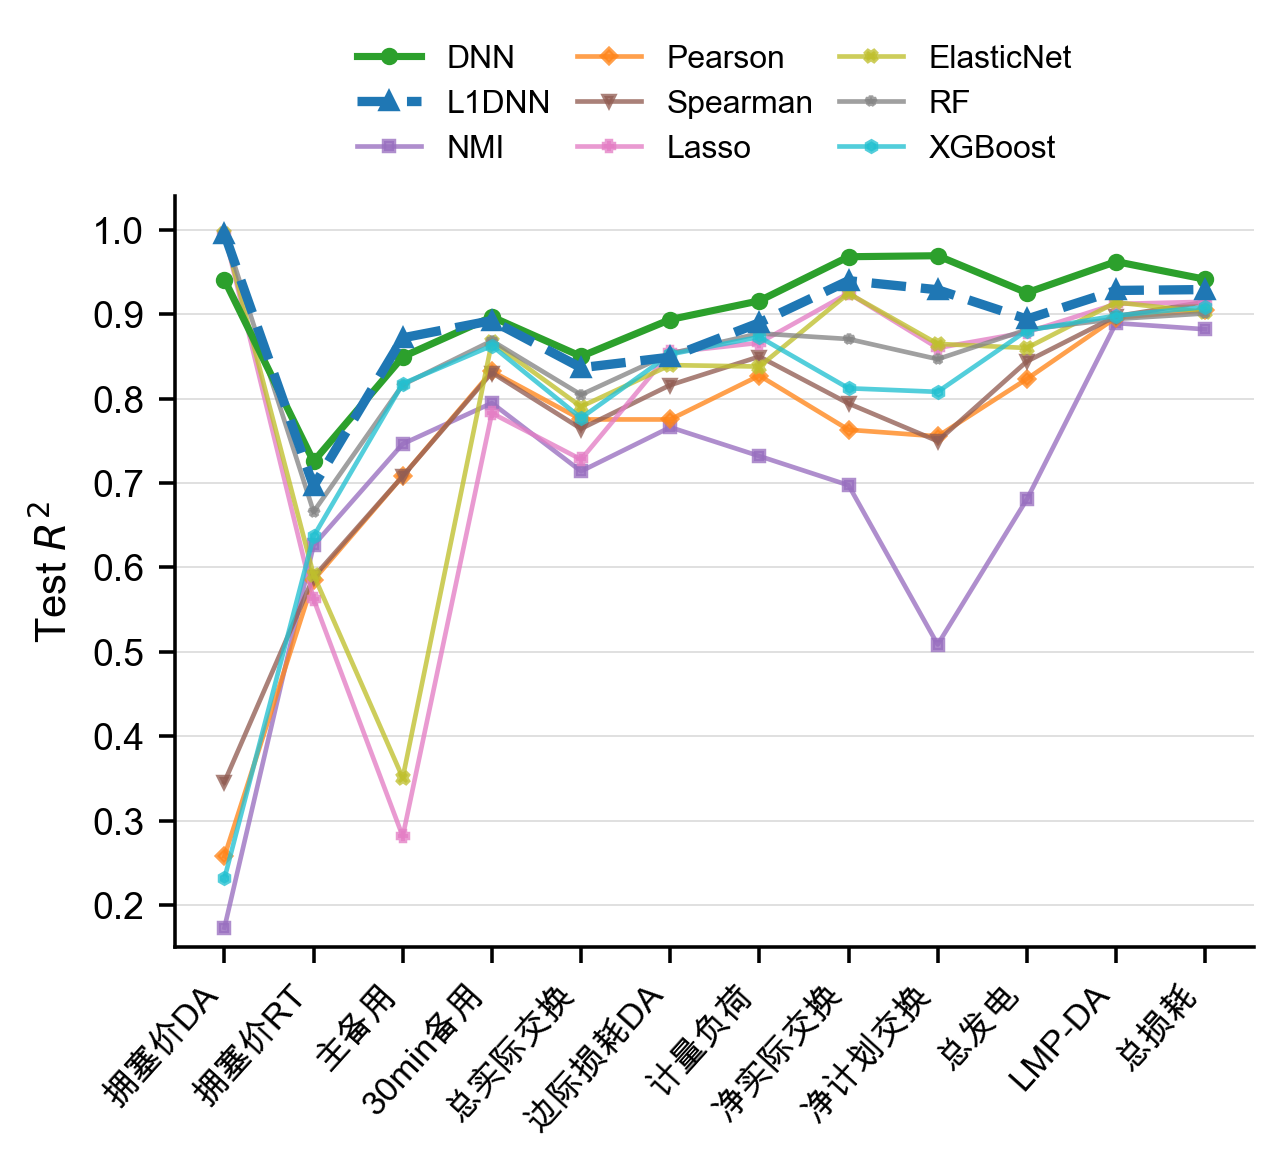
\includegraphics[width=\columnwidth]{budget95_baseline_lines_zh.png}\\[-0.2em]
{\scriptsize (a) 95\% 统一预算}\\[0.45em]
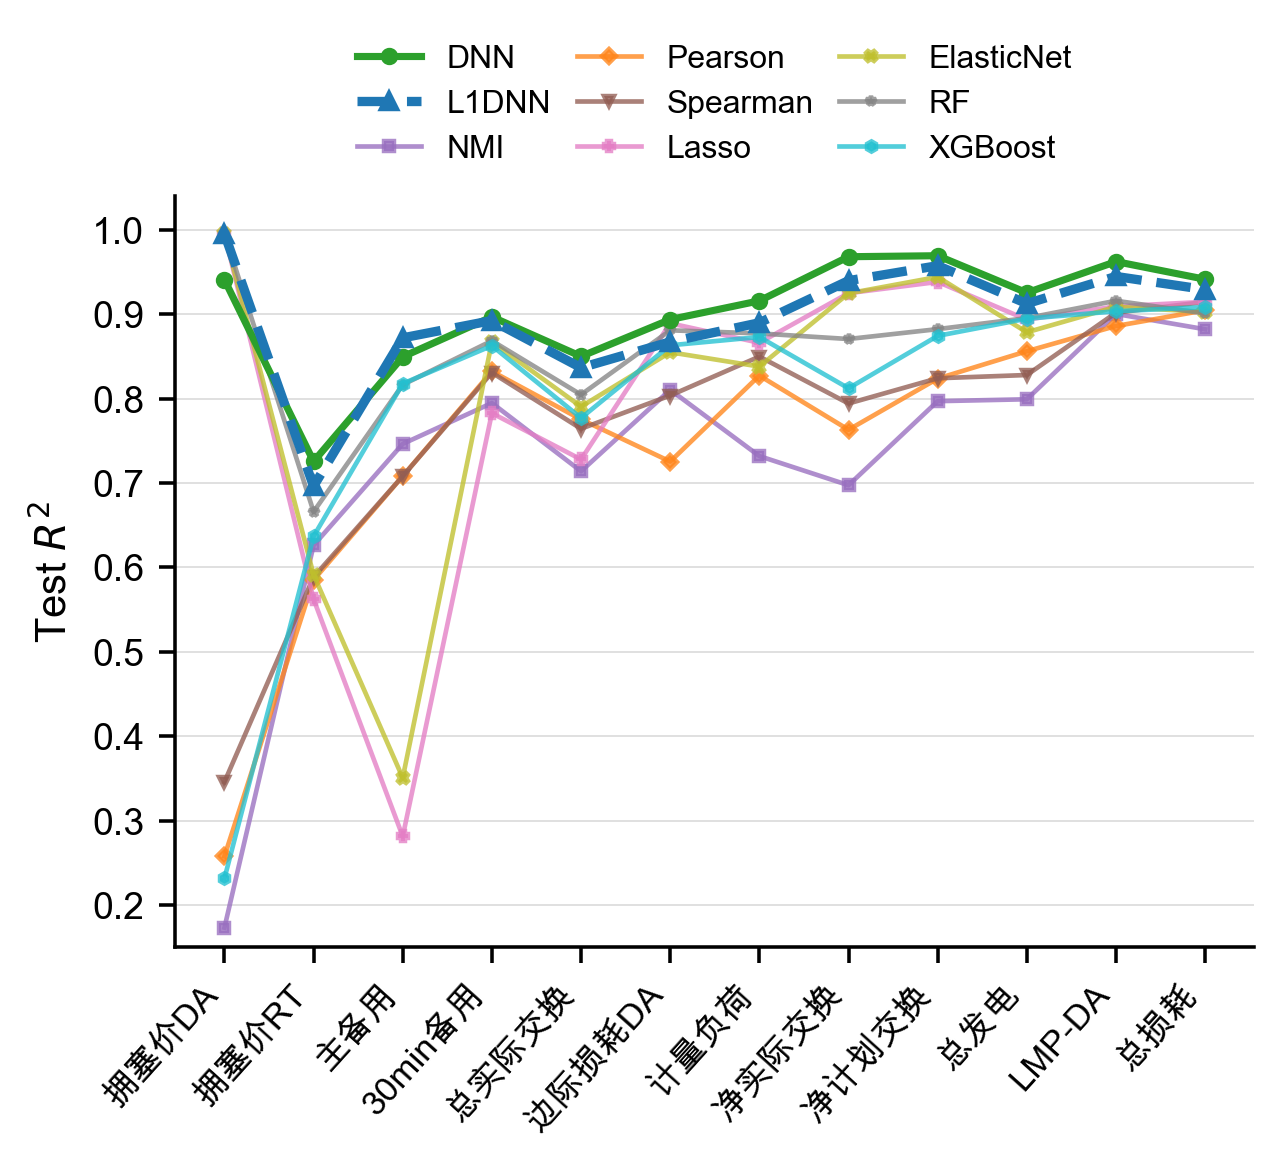
\includegraphics[width=\columnwidth]{budget97_baseline_lines_zh.png}\\[-0.2em]
{\scriptsize (b) 97\% 统一预算}
\figbicaption{统一预算下各目标的 baseline 测试 $R^2$ 对比}{Target-level baseline comparison under unified feature budgets}
\label{fig:budget_lines}
\end{figure}

\begin{figure}[!tbp]
\centering
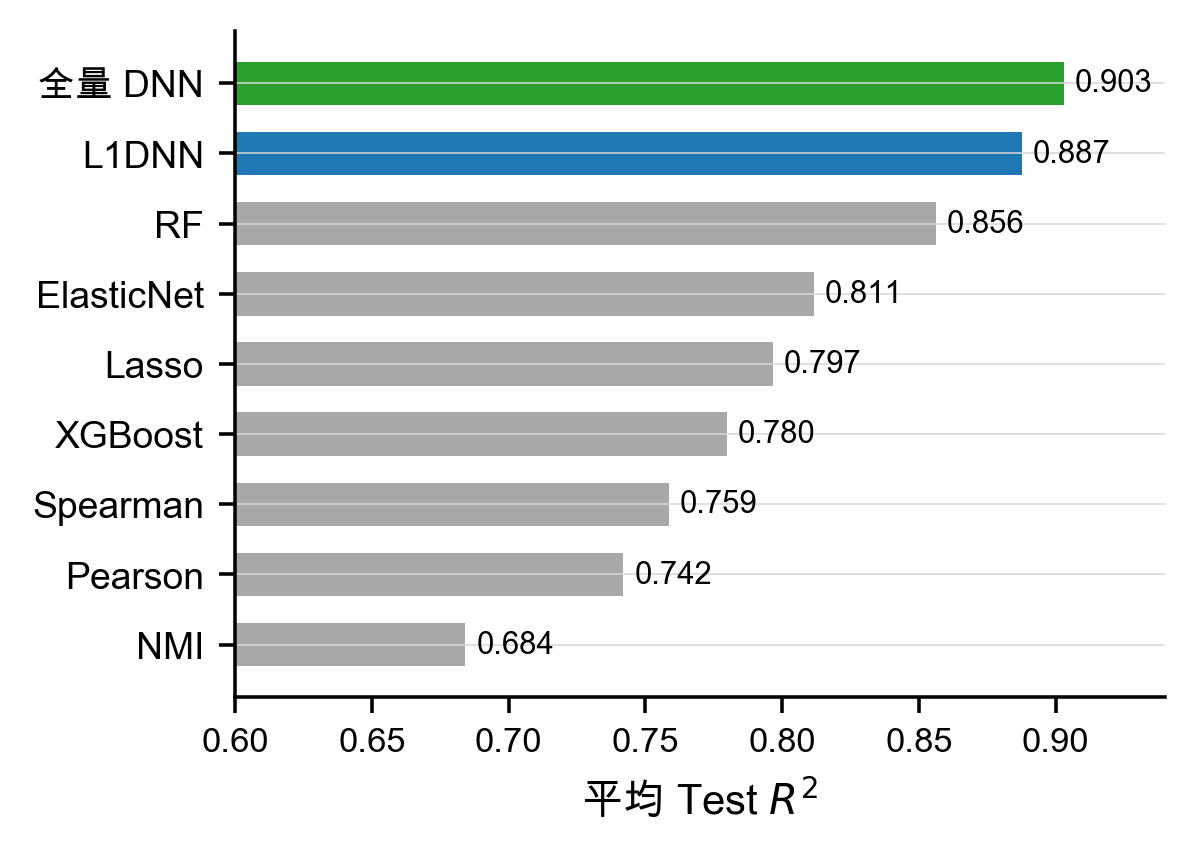
\includegraphics[width=\columnwidth]{budget95_average_bar_zh.png}\\[-0.2em]
{\scriptsize (a) 95\% 统一预算}\\[0.45em]
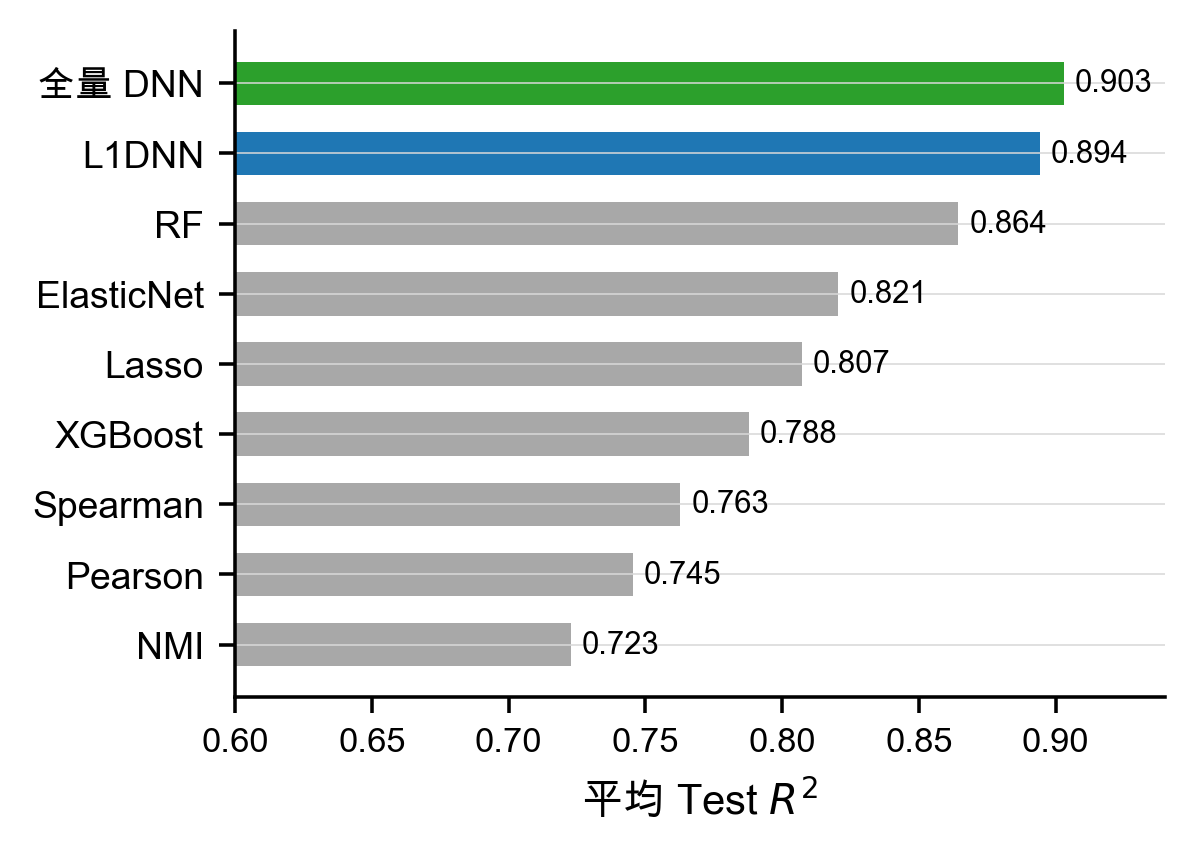
\includegraphics[width=\columnwidth]{budget97_average_bar_zh.png}\\[-0.2em]
{\scriptsize (b) 97\% 统一预算}
\figbicaption{统一预算下各 baseline 方法的平均测试 $R^2$}{Average test $R^2$ of baseline methods under unified feature budgets}
\label{fig:budget_avg}
\end{figure}

\subsection{冗余输入影响分析}
\subsubsection{训练曲线对比分析}
在上述实验中，部分目标出现了 L1 门控选中字段的测试 $R^2$ 高于全量字段 DNN 的现象。这一看似反直觉的结果并非意味着全量字段所含信息量不足，而是揭示了全量输入中冗余和噪声字段对深度模型泛化性能的负面影响。在高维输入空间中，普通多层感知器在有限样本条件下容易对弱相关字段产生过度拟合，表现为训练集拟合度持续提升而测试集泛化性能出现下降。

为验证上述分析，本文选取性能差异较为显著的日前拥塞价和主备用容量两个目标，对比全量 DNN、L1 门控模型和 L1 选中特征再训练 DNN 的训练曲线，结果如图~\ref{fig:redundant_curve} 和表~\ref{tab:noise_curve} 所示。

对于日前拥塞价目标，全量 DNN（69 字段）的最优测试 $R^2$ 为 0.9408，最终训练集与测试集的泛化差距约为 0.0621；而仅使用 L1 门控选出的 2 个字段重新训练普通 DNN 后，最优测试 $R^2$ 达到 0.9954，泛化差距大幅缩小至 0.0025。对于主备用容量目标，全量 DNN（67 字段）的泛化差距约为 0.1439，L1 选中特征 DNN（35 字段）的测试 $R^2$ 从 0.8495 提升至 0.8580，泛化差距也有所改善。上述结果表明，字段压缩有效降低了模型对弱相关和噪声字段的过度记忆，使模型在测试集上的表现更加稳定。

\begin{figure}[!tbp]
\centering
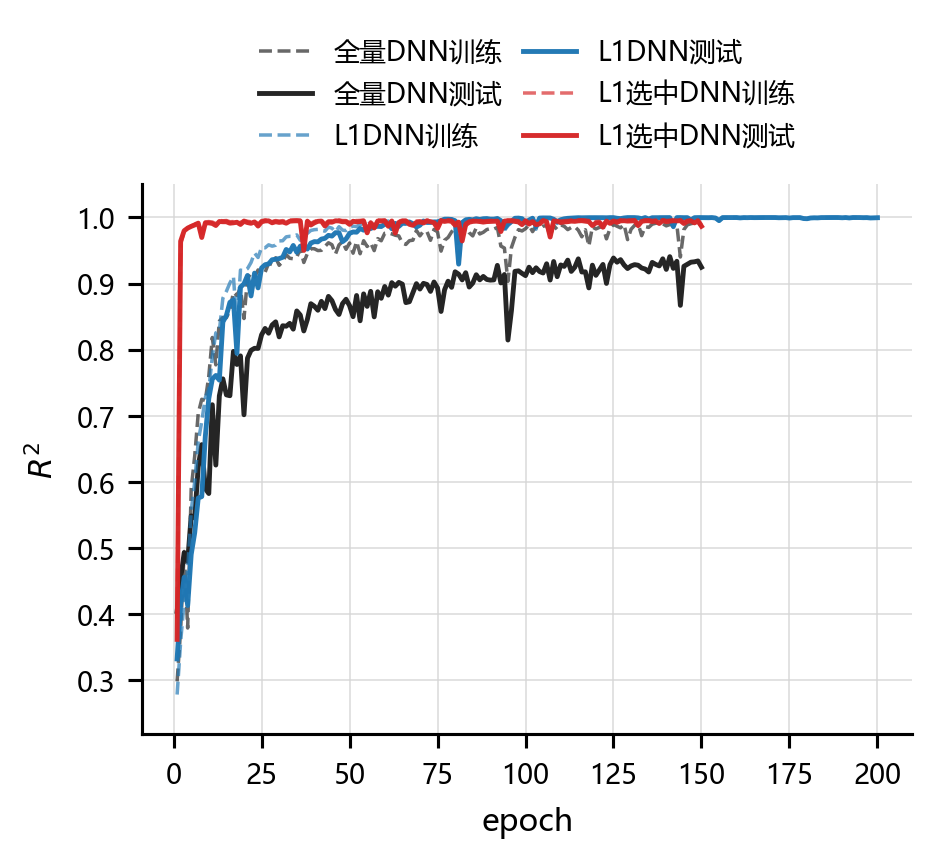
\includegraphics[width=\columnwidth]{redundant_training_congestion_zh.png}\\[-0.2em]
{\scriptsize (a) 日前拥塞价}\\[0.45em]
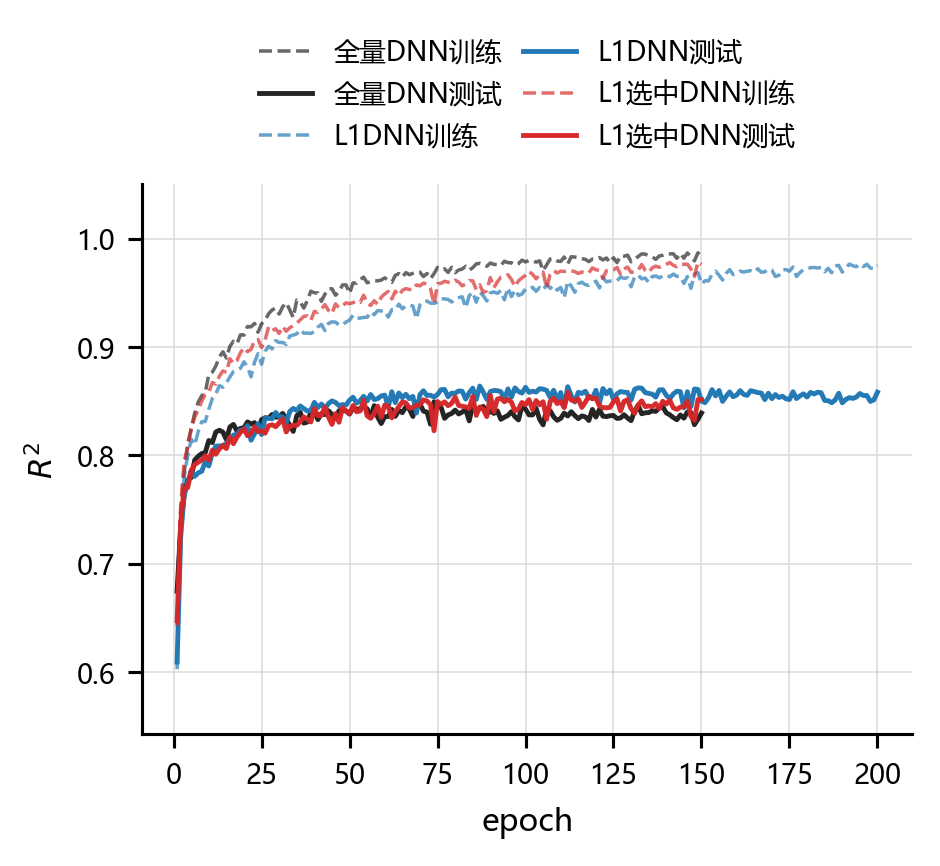
\includegraphics[width=\columnwidth]{redundant_training_primary_zh.png}\\[-0.2em]
{\scriptsize (b) 主备用容量}
\figbicaption{全量字段与 L1 选中特征的训练/测试 $R^2$ 曲线对比}{Comparison of train/test $R^2$ curves between all features and L1-selected features}
\label{fig:redundant_curve}
\end{figure}

\begin{table}[!tbp]
\centering
\scriptsize
\setlength{\tabcolsep}{3pt}
\tabbicaption{冗余噪声解释实验训练曲线统计}{Training-curve statistics for redundant-noise explanation}
\label{tab:noise_curve}
\textbf{(a) 日前拥塞价}\\[-0.2em]
\begin{tabularx}{\columnwidth}{Xrrrr}
\toprule
方法 & 字段数 & Best $R^2$ & epoch & 泛化差距 \\
\midrule
全量 DNN & 69 & 0.9408 & 141 & 0.0621 \\
L1GateDNN & 69 & 1.0000 & 194 & -0.0001 \\
L1 选中特征 DNN & 2 & 0.9954 & 139 & 0.0025 \\
\bottomrule
\end{tabularx}

\vspace{0.4em}
\textbf{(b) 主备用容量}\\[-0.2em]
\begin{tabularx}{\columnwidth}{Xrrrr}
\toprule
方法 & 字段数 & Best $R^2$ & epoch & 泛化差距 \\
\midrule
全量 DNN & 67 & 0.8495 & 74 & 0.1439 \\
L1GateDNN & 67 & 0.8639 & 87 & 0.1170 \\
L1 选中特征 DNN & 35 & 0.8580 & 112 & 0.1247 \\
\bottomrule
\end{tabularx}
\end{table}

\subsubsection{Top-n 递增实验}
为进一步揭示字段数量与推断性能之间的关系，本文按 L1 门控值排名逐步增加输入字段数，记录各组合下的测试 $R^2$。图~\ref{fig:topn_noise} 给出了日前拥塞价和主备用容量两个目标的完整 Top-n 序列结果，其中三角形标记表示 $R^2$ 最高点，方形标记表示全量字段对应的结果。

对于日前拥塞价目标，仅 Top2 字段即达到 0.9954 的测试 $R^2$，Top3 进一步提升至 0.9999，在 Top24 范围内均保持较高水平；然而当字段数增加至 Top32 时，$R^2$ 下降至 0.9851，全量 69 字段的结果仅为 0.9408。对于主备用容量目标，$R^2$ 随字段数从 Top1 到 Top24 逐步提升至 0.8872 的峰值，但继续增加至 Top32 和 Top35 后分别降至 0.8545 和 0.8536，接近全量 DNN 的 0.8495。

上述递增实验揭示了字段数量与推断性能之间的典型非单调关系：当关键字段不足时，模型缺乏必要的信息源，推断能力受限；当字段数量处于合理区间时，核心推断路径被充分激活，推断精度显著提升；而当冗余和弱相关字段继续加入后，输入空间的维度增大，模型更容易记忆训练样本中的扰动信息，导致泛化收益递减甚至出现逆转。这一发现说明，适度字段压缩并非简单减少信息量，而是在保留主要关联路径的同时降低冗余输入对模型训练的干扰。

\begin{figure}[!tbp]
\centering
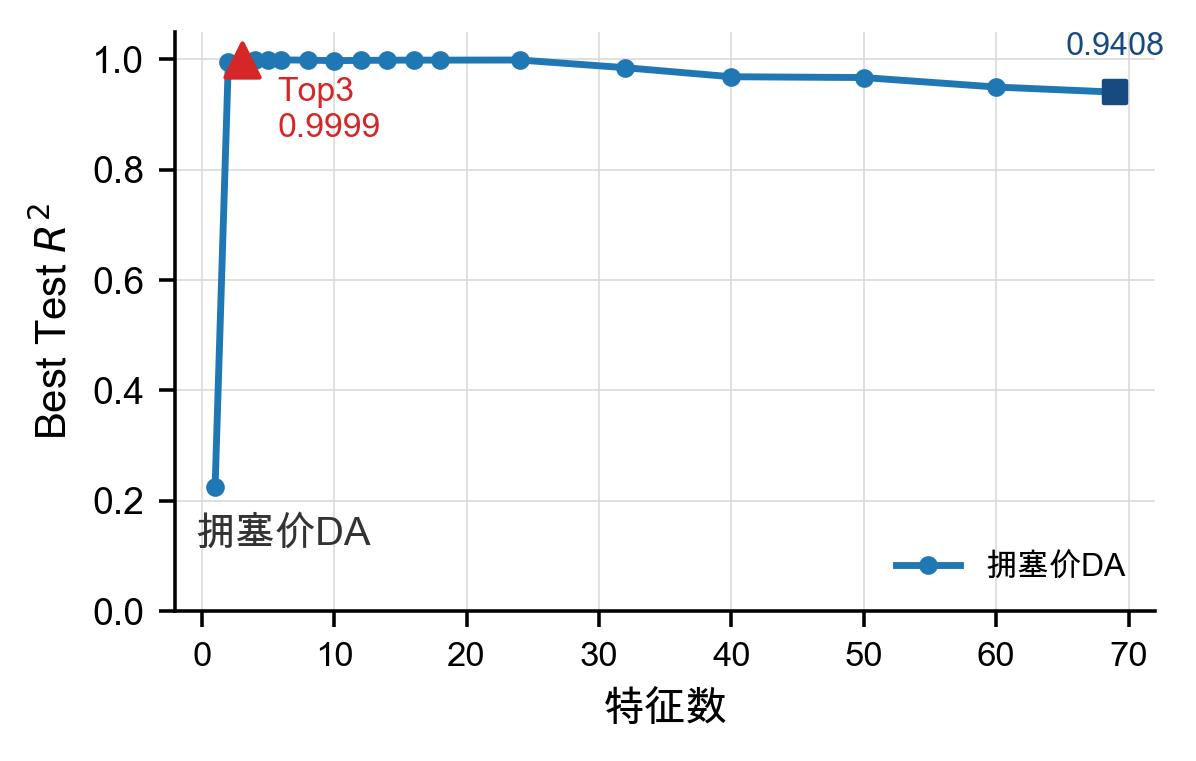
\includegraphics[width=\columnwidth]{topn_congestion_zh.png}\\[-0.2em]
{\scriptsize (a) 日前拥塞价}\\[0.45em]
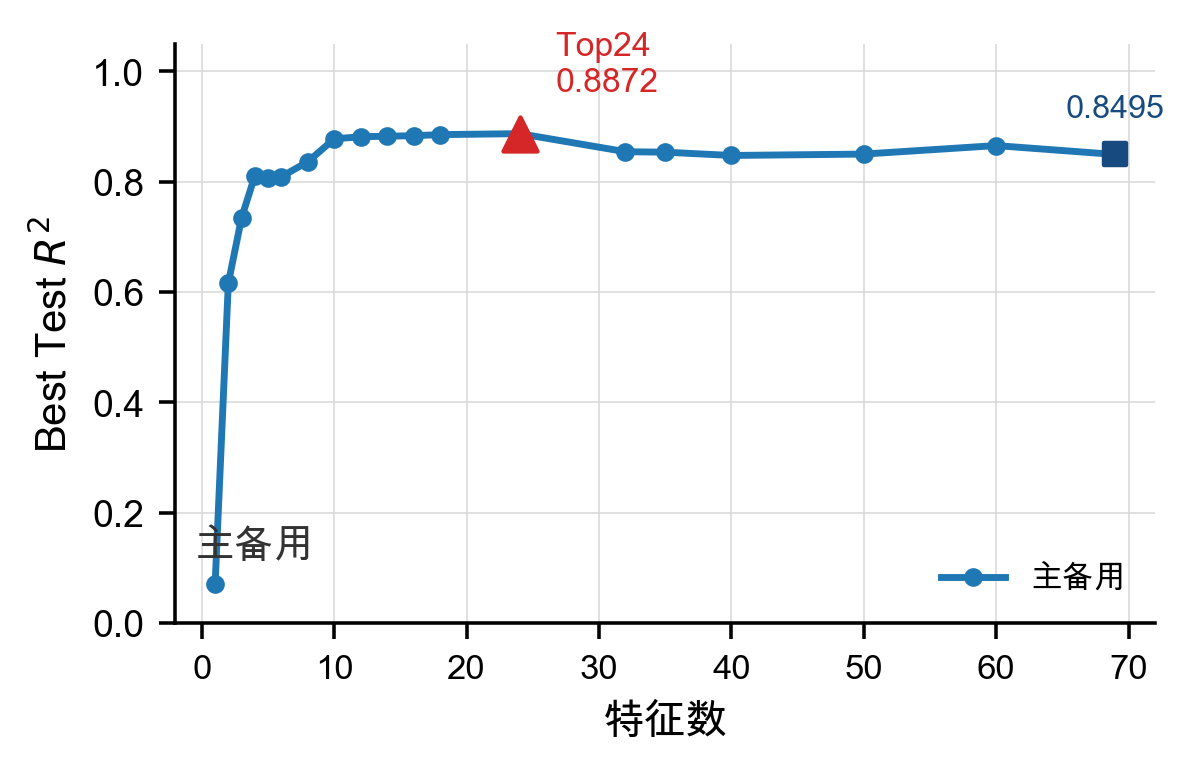
\includegraphics[width=\columnwidth]{topn_primary_zh.png}\\[-0.2em]
{\scriptsize (b) 主备用容量}
\figbicaption{按 L1 门控排名逐步增加字段数的测试 $R^2$ 变化}{Test $R^2$ variation with incrementally added Top-n features ranked by L1 gate values}
\label{fig:topn_noise}
\end{figure}

\section{讨论}
上述实验结果表明，所提 L1 门控方法的核心优势不仅体现在平均 $R^2$ 的数值提升，更在于其输出形式适合电力数据关联分析中的字段级解释需求。全量深度模型虽可证明目标变量整体可被预测，但无法定位具体的推断路径和关键贡献字段；单相关性分析方法可以量化字段间的两两关联强度，但无法判断各字段在联合推断中的不可替代性；线性稀疏模型和树模型能够给出特征重要性排序，但其排序标准与深度模型实际推断能力之间缺乏一致性保证。本文所提 L1 门控模型将字段选择嵌入非线性深度推断的训练过程中，使字段的保留或剔除直接受到预测误差和稀疏约束的联合驱动，因此其输出的活跃字段集合更接近“哪些字段实际支撑目标变量恢复”的推断语义。

同预算 baseline 对比实验进一步说明了统一字段预算策略的合理性。固定字段数 $n$ 并非为了偏向 L1 门控方法，而是为了构造公平且可解释的比较基准：若允许各方法自由选择不同数量的字段，则性能差异可能来源于字段数差异而非选择质量差异。本文在 95\% 和 97\% 两种预算水平下均开展了对比，既展示了较低容忍度下 L1 门控方法的领先优势，也揭示了在较高容忍度下各方法性能趋近全量 DNN 的收敛趋势。

少量字段推断精度优于全量字段的现象具有深层的实际含义。在电力数据中，大量字段并非独立信息源，而是由相同的物理过程或市场机制派生而来。将这些共线性强或弱相关的字段全部作为模型输入，会扩大输入空间维度，增大深度模型记忆训练样本细节的倾向，从而影响测试集泛化表现。L1 门控通过在训练过程中先行筛选出稳定推断路径，再由普通 DNN 独立验证其推断能力，实质上实现了输入维度的合理压缩和冗余输入影响控制。因此，字段压缩的本质并非信息舍弃，而是在保留核心推断路径的同时消除冗余噪声的干扰。

本文研究仍存在以下局限性。第一，L1 正则化系数和活跃阈值的选择会影响最终的字段筛选结果，在实际应用中应根据字段规模、噪声水平和分析目的进行调整。第二，部分目标变量可能存在多条等价推断路径，单次训练得到的活跃字段集合不一定唯一，后续研究应引入多随机种子和跨时间窗口的稳定性分析机制。第三，本文以单目标推断为中心构建分析框架，多目标之间的联合关联结构和推断路径传播机制尚待进一步研究。

\section{结论}
本文围绕高维电力数据中的隐性推断源定位问题，提出了融合多相关性筛选与 L1 门控深度神经网络的分析方法。该方法首先通过六类统计指标对候选字段进行多维度依赖性初筛，尽量保留不同类型的潜在关联字段；随后利用 L1 门控深度神经网络在保持目标变量推断能力的前提下自动压缩冗余字段，获取紧凑的活跃推断源集合；进而通过普通深度神经网络再训练独立验证所选字段的实际推断能力。此外，本文构建的相关性驱动改进门控模型将六类统计指标映射为统一的门控判定边界，增强了分析方法的可解释性。

基于美国 PJM 电力市场 2025 年小时级运行数据的实验结果表明：针对净实际交换功率目标，所提方法从 55 个候选字段中筛选出 18 个活跃字段，以此训练的普通 DNN 验证 $R^2$ 为 0.9681，高于全量字段结果 0.9661，而未选中字段单独推断仅为 0.7820。在 12 个目标变量上，L1 门控模型以平均 15.5 个字段（字段利用率约 22.46\%）取得 0.9111 的平均测试 $R^2$，高于全量 DNN 的 0.9031。在 95\% 和 97\% 同预算 baseline 对比中，L1 门控方法在各预算水平下均保持最优平均 $R^2$。冗余输入影响分析进一步揭示了全量输入中弱相关和冗余字段可能降低泛化表现的现象，为合理的字段压缩策略提供了实证依据。上述结果表明，所提方法能够有效定位电力数据中的隐性推断路径和关键贡献字段，可为电力数据关联解释、字段分级和共享前评估提供技术支撑。

未来研究将从以下三个方面展开：一是引入多随机种子和跨月份时间窗口验证，评估门控字段集合的跨场景稳定性；二是将单目标推断分析扩展为多目标关联图谱构建，系统刻画不同目标变量之间的联合推断关系和路径传播规律；三是将识别出的推断源集合与字段降精度、延迟发布和分级授权等数据处置策略相结合，构建面向实际电力数据共享流程的闭环评估机制。

\balance
\begin{thebibliography}{99}
\bibitem{ref-liu-cps}
刘涛, 田捷, 王杰, 等. 信息物理融合系统的综合安全威胁与防御研究[J]. 自动化学报, 2019, 45(1): 5-24.

LIU Tao, TIAN Jie, WANG Jie, et al. Integrated security threats and defense of cyber-physical systems[J]. Acta Automatica Sinica, 2019, 45(1): 5-24.

\bibitem{ref-ma-pjm}
马珍, 张弘, 朱兰, 等. 美国电力市场信息披露制度及其对中国的启示[J]. 电力系统自动化, 2017, 41(24): 49-57.

MA Zhen, ZHANG Hong, ZHU Lan, et al. Information disclosure system in American electricity market and its enlightenment for China[J]. Automation of Electric Power Systems, 2017, 41(24): 49-57.

\bibitem{ref-fan-pjm}
Fan Z, Horger T, Bastian J, et al. An overview of PJM energy market design and development[C]//2008 Third International Conference on Electric Utility Deregulation and Restructuring and Power Technologies. Piscataway: IEEE, 2008: 12-17.

\bibitem{ref-sankar}
Sankar L, Rajagopalan S R, Mohajer S, et al. Smart meter privacy: A theoretical framework[J]. IEEE Transactions on Smart Grid, 2013, 4(2): 837-846.

\bibitem{ref-giaconi}
Giaconi G, Gündüz D, Poor H V. Privacy-aware smart metering: Progress and challenges[J]. IEEE Signal Processing Magazine, 2018, 35(6): 59-78.

\bibitem{ref-adewole}
Adewole K S, Torra V. Privacy issues in smart grid data: From energy disaggregation to disclosure risk[C]//International Conference on Database and Expert Systems Applications. Cham: Springer, 2022: 71-84.

\bibitem{ref-lan-load}
兰丁, 朱慧, 吴杰, 等. 基于改进 AlexNet-GRU 深度学习网络的配电网短期负荷预测方法[C]//2021 IEEE 5th Conference on Energy Internet and Energy System Integration. Piscataway: IEEE, 2021: 3004-3010.

LAN Ding, ZHU Hui, WU Jie, et al. A short-term load forecasting method of distribution network based on improved AlexNet-GRU deep learning network[C]//2021 IEEE 5th Conference on Energy Internet and Energy System Integration. Piscataway: IEEE, 2021: 3004-3010.

\bibitem{ref-jiao-pv}
焦鑫, 孙源, 彭迪, 等. 基于方差变点与相关性分析的光伏功率异常数据清洗[C]//2021 6th International Conference on Power and Renewable Energy. Piscataway: IEEE, 2021: 1140-1145.

JIAO Xin, SUN Yuan, PENG Di, et al. Photovoltaic power abnormal data cleaning based on variance change point and correlation analysis[C]//2021 6th International Conference on Power and Renewable Energy. Piscataway: IEEE, 2021: 1140-1145.

\bibitem{ref-deng-load}
邓鑫, 张超, 彭辉, 等. 基于相关性分析与特征提取的区域电网短期负荷预测[C]//2022 7th Asia Conference on Power and Electrical Engineering. Piscataway: IEEE, 2022: 1081-1085.

DENG Xin, ZHANG Chao, PENG Hui, et al. Short-term load forecasting for regional power grids based on correlation analysis and feature extraction[C]//2022 7th Asia Conference on Power and Electrical Engineering. Piscataway: IEEE, 2022: 1081-1085.

\bibitem{ref-szekely-dcorr}
Székely G J, Rizzo M L, Bakirov N K. Measuring and testing dependence by correlation of distances[J]. The Annals of Statistics, 2007, 35(6): 2769-2794.

\bibitem{ref-gretton-hsic}
Gretton A, Bousquet O, Smola A, et al. Measuring statistical dependence with Hilbert-Schmidt norms[C]//Algorithmic Learning Theory. Berlin: Springer, 2005: 63-77.

\bibitem{ref-wang-meter}
Wang Y, Chen Q, Hong T, et al. Review of smart meter data analytics: Applications, methodologies, and challenges[J]. IEEE Transactions on Smart Grid, 2019, 10(3): 3125-3148.

\bibitem{ref-breiman-rf}
Breiman L. Random forests[J]. Machine Learning, 2001, 45(1): 5-32.

\bibitem{ref-chen-xgboost}
Chen T, Guestrin C. XGBoost: A scalable tree boosting system[C]//Proceedings of the 22nd ACM SIGKDD International Conference on Knowledge Discovery and Data Mining. New York: ACM, 2016: 785-794.

\bibitem{ref-tibshirani-lasso}
Tibshirani R. Regression shrinkage and selection via the lasso[J]. Journal of the Royal Statistical Society: Series B, 1996, 58(1): 267-288.

\bibitem{ref-zou-enet}
Zou H, Hastie T. Regularization and variable selection via the elastic net[J]. Journal of the Royal Statistical Society: Series B, 2005, 67(2): 301-320.

\bibitem{ref-xing-micdnn}
邢治, 王征, 冯健, 等. MIC-DNN：电力数据关联分析框架[C]//2025 40th Youth Academic Annual Conference of Chinese Association of Automation. Piscataway: IEEE, 2025: 2969-2974.

XING Zhi, WANG Zheng, FENG Jian, et al. MIC-DNN: Data-driven correlation analysis framework for power data[C]//2025 40th Youth Academic Annual Conference of Chinese Association of Automation. Piscataway: IEEE, 2025: 2969-2974.

\bibitem{ref-zhang-sgcc}
张伯明, 孙宏斌, 吴文传, 等. 智能电网控制中心的信息安全问题[J]. 南方电网技术, 2012, 6(2): 1-7.

ZHANG Boming, SUN Hongbin, WU Wenchuan, et al. Information security issues in smart grid control centers[J]. Southern Power System Technology, 2012, 6(2): 1-7.

\bibitem{ref-chen-privacy}
陈颖, 王科, 朱涛, 等. 电力大数据隐私保护技术综述[J]. 电力系统自动化, 2021, 45(14): 157-168.

CHEN Ying, WANG Ke, ZHU Tao, et al. Review on privacy-preserving technologies for power big data[J]. Automation of Electric Power Systems, 2021, 45(14): 157-168.

\bibitem{ref-lecun-deep}
LeCun Y, Bengio Y, Hinton G. Deep learning[J]. Nature, 2015, 521(7553): 436-444.

\bibitem{ref-goodfellow-deep}
Goodfellow I, Bengio Y, Courville A. Deep learning[M]. Cambridge: MIT Press, 2016.

\bibitem{ref-he-dropout}
Srivastava N, Hinton G, Krizhevsky A, et al. Dropout: A simple way to prevent neural networks from overfitting[J]. The Journal of Machine Learning Research, 2014, 15(1): 1929-1958.

\bibitem{ref-kingma-adam}
Kingma D P, Ba J. Adam: A method for stochastic optimization[C]//International Conference on Learning Representations. San Diego: ICLR, 2015.

\bibitem{ref-reshef-mic}
Reshef D N, Reshef Y A, Finucane H K, et al. Detecting novel associations in large data sets[J]. Science, 2011, 334(6062): 1518-1524.

\bibitem{ref-cover-info}
Cover T M, Thomas J A. Elements of information theory[M]. 2nd ed. Hoboken: John Wiley \& Sons, 2006.

\bibitem{ref-pjm-dataminer}
PJM Interconnection. PJM Data Miner 2[EB/OL]. [2025-05-01]. https://dataminer2.pjm.com.

\bibitem{ref-zhu-sharing}
朱涛, 陈颖, 张宁, 等. 面向电力数据共享的安全机制研究[J]. 中国电机工程学报, 2020, 40(S1): 21-30.

ZHU Tao, CHEN Ying, ZHANG Ning, et al. Security mechanisms for power data sharing[J]. Proceedings of the CSEE, 2020, 40(S1): 21-30.
\end{thebibliography}

\section*{收稿日期与作者简介}
\noindent\textbf{收稿日期：}20XX-XX-XX

\noindent\textbf{作者简介：}\par
\noindent 杜浩存（出生年），男，研究方向为电力数据安全、信息物理系统安全与机器学习安全，邮箱：待补充。

\end{document}
